\documentclass[11pt]{article}

%减少左右空白边缘
%\usepackage{fullpage}
\usepackage[left=1.3in, right=1.3in, top=1.3in, bottom=1.3in]{geometry}
%插入图像 .jpg .png .pdf
\usepackage{graphicx}
%支持中文
\usepackage[UTF8, heading = false, scheme = plain]{ctex}
% 页眉页脚
\usepackage{fancyhdr}
\pagestyle{fancy}
\fancyhead{}
\fancyfoot{}
\fancyhead[L]{\slshape Left Title}
\fancyhead[R]{\slshape Right Title}
\fancyfoot[C]{\thepage}

\begin{document}

% 标题页
\begin{titlepage}
\begin{center}

	\huge{\textbf{软件工程\ 课程设计报告}}\\

	\vfill
	\line(1, 0){400} \\ [1mm]
	\large{\textbf{09015116\ 樊博杰}} \\ [1mm]
	\large{\textbf{09015124\ 邹家伦}} \\ [1mm]
	\large{\textbf{09015128\ 张敏学}} \\ [1mm]
	\large{\textbf{09015204\ 杨艳春}} \\ [1mm]
	\large{\textbf{09015209\ 刘韦}} \\ [1mm]
	\line(1, 0){400} \\
	\large{\today}\\
\end{center}
\end{titlepage}

%目录
\tableofcontents
\thispagestyle{empty}
\clearpage


\setcounter{page}{1}
\fancyhead[R]{\slshape 用例与需求分析}
\section{用例与需求分析}
   缤客(Booking.com)是一家可以帮用户在网上预订世界各地住宿的网站。向用户提供各种类型住宿最优惠的价格,其中既有小型的家庭经营住宿加早餐旅馆,也有五星级豪华酒店。致力于提供信息全面且易于使用的网站以及最优惠价格保证。目标是为世界各地的商务人士和休闲旅客提供最易于使用且最实惠的方式,搜索并预订各种类型的住宿。公司的多语种客户服务团队致力于为所有的客人提供协助和支持。
	\subsection{参与者}
	一共有三类参与者: 酒店合作伙伴(Partner), 管理员(Administrator), 以及顾客(User)
	\subsection{分销合作伙伴 Partner}
		针对分销合作伙伴,booking网站提供了注册登录,访问酒店后台,更新日历,房价及其他设置,上线接受预定等功能。
		\subsubsection{注册登录}
		booking提供的注册功能,可以让用户注册成为分销合作伙伴,用户可以用邮箱注册,完成注册后,将审核用户提交的相关信息,确保信息正确完整。一旦通过审核,用户将收到邮件,内附“酒店后台”的登录信息。随后,合作伙伴还将收到操作指南
		\subsubsection{访问酒店后台}
		“酒店后台”是为合作伙伴提供的住宿管理系统。合作伙伴可用于编辑修改房量、房价等信息。
		\subsubsection{上线接受预定}
		完成注册审核后,会发送邮件,告知贵住宿在Booking.com上线的后续步骤。订单即时确认
        	所有来自Booking.com的客人订单均为即时确认,为酒店合作伙伴省心省力。
        	\subsubsection{24小时客户支持}
        	当地支持团队全天24小时为酒店提供协助,支持41种语言。
        	\subsubsection{酒店评论查看与回复}
        	评语审核团队将对所有客人评语进行核查,只有客人实际入住了预订的酒店,提交的评语方可显示在网站上。这样的评语更有可信度,能够为酒店吸引更多客人。合作伙伴可以查看有关酒店的评语,并进行回复。
	\subsection{管理员 Administrator}
        针对 BOOKING 网站管理员,BOOKING 主要提供了登录,管理用户,提供推送,在线客服等主要功能。 
        	\subsubsection{登陆}
        	管理员可以凭借管理员账号登陆 BOOKING 网站,获得管理权限。 
        	\subsubsection{管理用户}  
        	管理员可以审核酒店合作伙伴的注册信息,通过或拒绝申请。也可以对行为不当的用户进行删除或者封号。对注册成功的酒店合作伙伴账号进行删除或封号。 
        	\subsubsection{提供推送}
        	管理员可以根据热门的旅游地点,旅游主题,优惠折扣等发布推荐,更新常见问题列表,发布最新 新闻,发布招聘信息等一系列的推送。 
        	\subsubsection{在线客服}  
        	管理员可以查看来自酒店合作伙伴和普通用户的建议或提问,可以给出回复,并且可以查看用户对在线客服的评价。
		\subsubsection{订单修改} 
		管理员可按用户的需求帮助用户修改订单。
		
	\subsection{顾客 User}
		针对普通用户, booking 网站提供了注册登录, 酒店搜索和预订, 评论, 设置等功能
		\subsubsection{注册登录}
		booking 提供的注册功能可以让游客注册成为用户,用户可以用已有账号登录,微信登录,或绑定其他的社交账号,例如 Google,Facebook 等。
		\subsubsection{查看推送}
		booking 会根据热门的旅游主题,旅游地点,优惠折扣,用户所在地等推荐相关的酒店,并且提供详细的酒店信息。用户可以随时查看最热门的推送消息,选择合适的酒店。
		\subsubsection{酒店搜索}
		booking 提供的搜索功能可以根据目的地、住宿名称或地址,针对住宿时间、出行类别、客房数量、随行人数等查询有空余房间的符合条件的酒店。booking 非常贴心的根据全球驴友的出行记录和喜好为用户提供了根据旅行关键词和地点搜索受欢迎的酒店。在通过目的地搜索时,用户可以选择使用地图浏览模式,更直观便捷。搜索完成后,booking 系统优先显示热门推荐酒店和网友推荐旅行主题,用户可以选择按价格、评分、距离市中心远近、星级等进行排序。并且可以通过一些筛选类别来缩小搜索范围,筛选类别有:每晚房价、热门筛选、住宿房量、住宿评级、住处类型、设施、餐点、预定政策、优惠、评分、床型偏好、24 小时前台、热门主题/活动、海滩、客房设施、酒店所在区、连锁酒店。针对用户选择的酒店,具体提供了以下信息:酒店星级、酒店价格、酒店照片、相关文字介绍、用户评论、在地图上的位置、推荐的精彩活动、可预订空房列表、设施、相关条款、预订须知等,并会根据用户点评提炼出关键词。用户可以选择咨询客服、将酒店添加至心愿单、立刻预订、分享给好友。
		\subsubsection{酒店预订}
			用户搜索到符合条件的酒店,网站会展示酒店信息的图文及游客的评价,供用户全面了解酒店的信息;若决定立即预定,用户将要填写自己的个人信息和自己的进一步详细需求,输入银行卡号,用户暂时无需付款。但住宿提供方可能会暂时冻结银行卡内的部分金额,以测试银行卡有效性并担保订单。这部分金额稍后将会退还。最后完成预定。
		
		\subsubsection{浏览记录}
		用户在浏览 booking 网站时,网站会提供用户的最新浏览记录,浏览该酒店的人数,最新的用户评论,最新订单等实时信息。
		
        \subsubsection{评语}
        用户可以对入住的酒店进行评价,或推荐,也可参与旅行问答,编写的评语将会转至待审核的评语栏等待工作人员审核。
        \subsubsection{我的收藏}
        用户可以将心仪的住宿保存至收藏列表,方便之后查找;也可分享自己的收藏那个,或创建新的心愿单。
        \subsubsection{个人设置}
        用户可在个人设置中完善自己的个人信息,预订信息和银行卡信息;进行支付设置,选择不同的支付方式;用户也可设置旅游偏好,便于网站提供给用户个性化的推荐。
		
		




\pagebreak
\fancyhead[R]{\slshape 用例图, 事件流, 类图, 顺序图, 状态图}
\section{用例图, 事件流, 类图, 顺序图, 状态图}



	\subsection{用户管理}
	
		\subsubsection{注册}
			用例: \\ \\
			\begin{tabular}{c|l}
			\hline
			用例名称 & 注册Register \\ \hline
			参与者 & 酒店合作伙伴Partner, 顾客User  \\ \hline
			入口条件 & 用户点击注册按钮 \\ \hline
			事件流 & 	\parbox{33em}{\ \\
						1. 用户点击注册按钮 \\
						2. 系统弹出注册窗口, 用户在窗口中输入账号, 密码, 确认密码, 邮箱, 手机号等信息, 选择注册类型(Partner, User), 点击确认  \\
						3. 系统弹出验证码输入窗口 \\
						4. 用户点击获取验证码, 系统向手机号或邮箱发送验证码 \\
						5. 用户输入验证码, 点击确认 \\
						6. 注册成功. 系统提示注册成功, 并向邮箱发送注册成功的邮件 \\
						} \\ \hline
			出口条件 & 注册成功或用户主动退出 \\ \hline
			质量需求 & \parbox{33em}{\ \\
						1. 用户两次输入的密码相匹配, 邮箱, 手机号格式正确 \\ 
						2. 用户名未被注册 \\
						3. 验证码须在10min之内成功验证 \\
						4. 网络通畅 \\
						} \\ \hline
			\end{tabular}\\ \\ \\
			\texttt{
			Algorithm Register \\
			Input : username, password, email, phoneNumber \\
			Output : true or false \\
			1. find the same username in database \\
			2. if(username is exist) \\
			3.     return false \\
			4. return true \\
			} \\
			
			语言成分分析:
			\begin{center}
			\begin{tabular}{|c|c|c|}
			\hline
			语言成分 & 模型构件 & 实例\\ \hline
			专有名词 & Object & Jack  \\ \hline
			普通名词 & Class & 用户, 界面 \\ \hline
			Doing 动词 & Method &  修改, 注册 \\ \hline
			Having 动词 & aggregation & 包括 \\ \hline
			形容词, 名词 & Attribute & 用户名,密码,邮箱,手机号码 \\ \hline
			\end{tabular}
			\end{center}
			
			用例图: 
			\begin{center}
			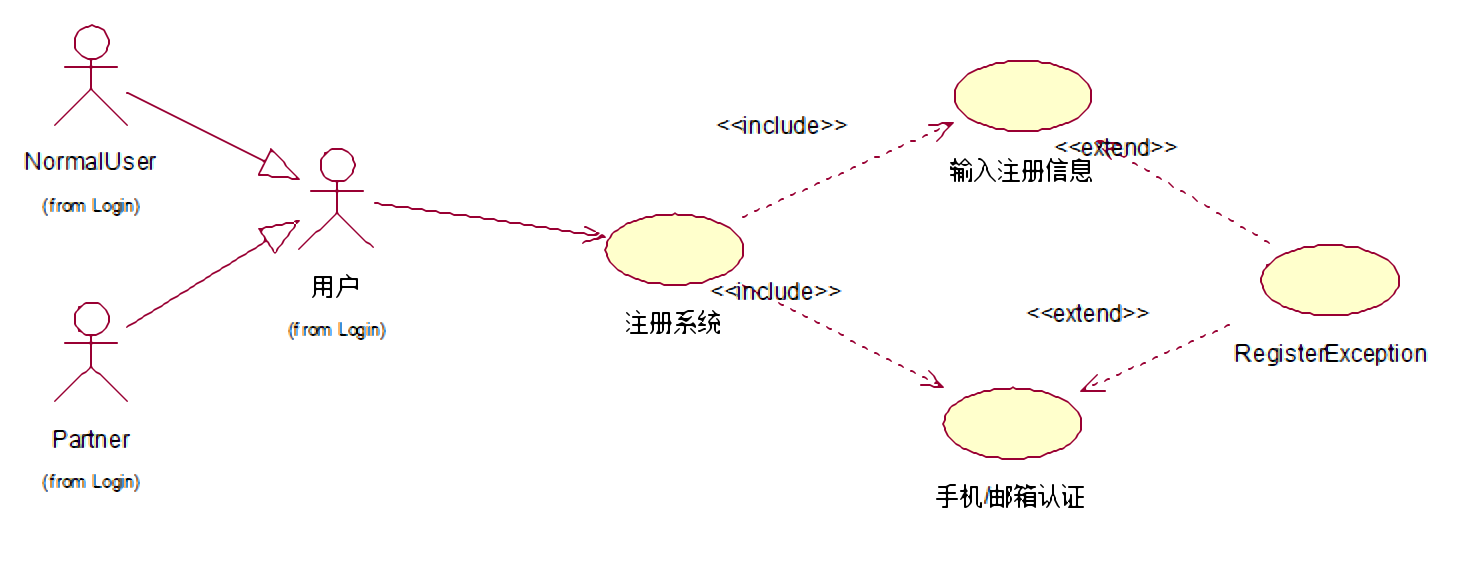
\includegraphics[scale=0.42]{注册_用例图.png}
			\end{center}

			类图: 
			\begin{center}
			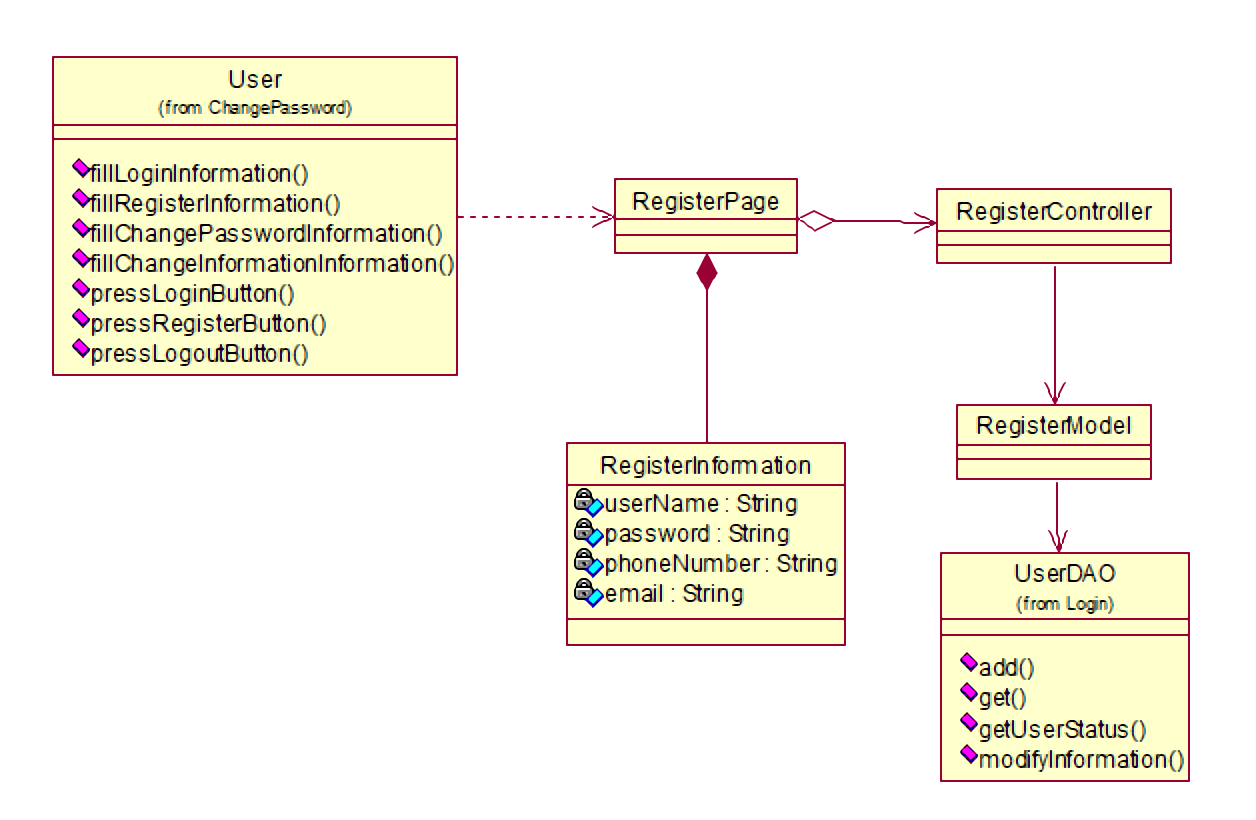
\includegraphics[scale=0.42]{注册_类图.png}
			\end{center}

			状态图: 
			\begin{center}
			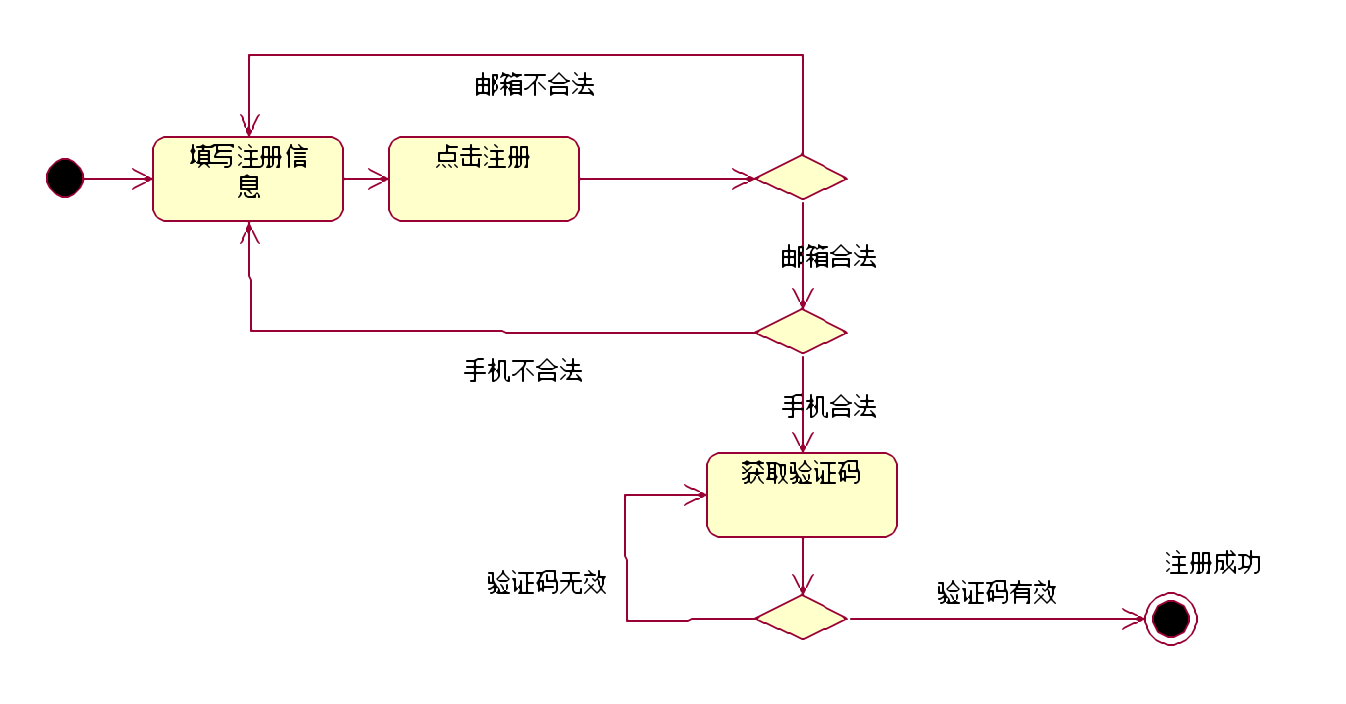
\includegraphics[scale=0.42]{注册_状态图.png}
			\end{center}

			顺序图: 
			\begin{center}
			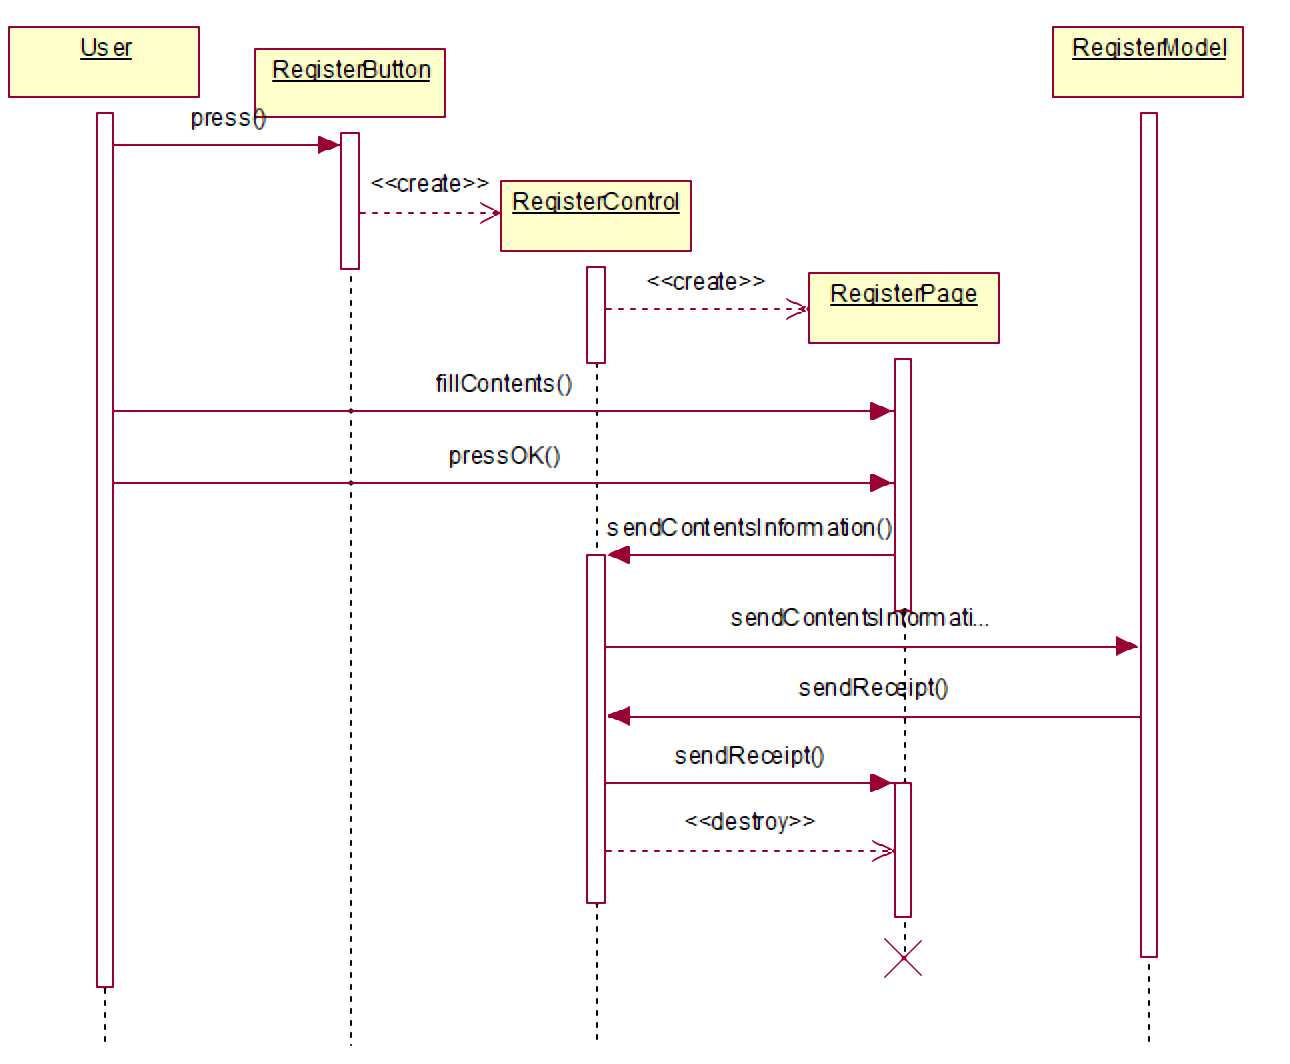
\includegraphics[scale=0.42]{注册_顺序图.png}
			\end{center}



		\subsubsection{登录}
			用例: \\ \\
			\begin{tabular}{c|l}
			\hline
			用例名称 & 登录 login \\ \hline
			参与者 & 酒店合作伙伴Partner, 管理员Administrator, 以及顾客User  \\ \hline
			入口条件 & 用户点击登录按钮 \\ \hline
			事件流 & 	\parbox{33em}{\ \\
						1. 用户点击登录按钮 \\
						2. 系统弹出登录窗口 \\
						3. 用户在窗口中输入账号, 密码和验证码, 点击确认  \\
						4. 系统在后台验证用户输入的账号, 密码以及验证码的正确性 \\
						5. 登录成功 \\
						} \\ \hline
			出口条件 & 登录成功或用户主动退出 \\ \hline
			质量需求 & \parbox{33em}{\ \\
						1. 用户输入的账号和密码相匹配 \\
						2. 用户输入的验证码正确 \\
						} \\ \hline
			\end{tabular}\\ \\ \\
			\texttt{
			Algorithm Login \\
			Input : username, password \\
			Output : true or false \\
			1. find the same username in database \\
			2. if(username is exist and password is right) \\
			3.     return true \\
			4. return false \\
			} \\
			
			语言成分分析:
			\begin{center}
			\begin{tabular}{|c|c|c|}
			\hline
			语言成分 & 模型构件 & 实例\\ \hline
			专有名词 & Object & Jack  \\ \hline
			普通名词 & Class & 用户,界面 \\ \hline
			Doing 动词 & Method &  修改,登录 \\ \hline
			Having 动词 & aggregation & 包括 \\ \hline
			形容词, 名词 & Attribute & 用户名,密码 \\ \hline
			\end{tabular}
			\end{center}
			
			用例图: 
			\begin{center}
			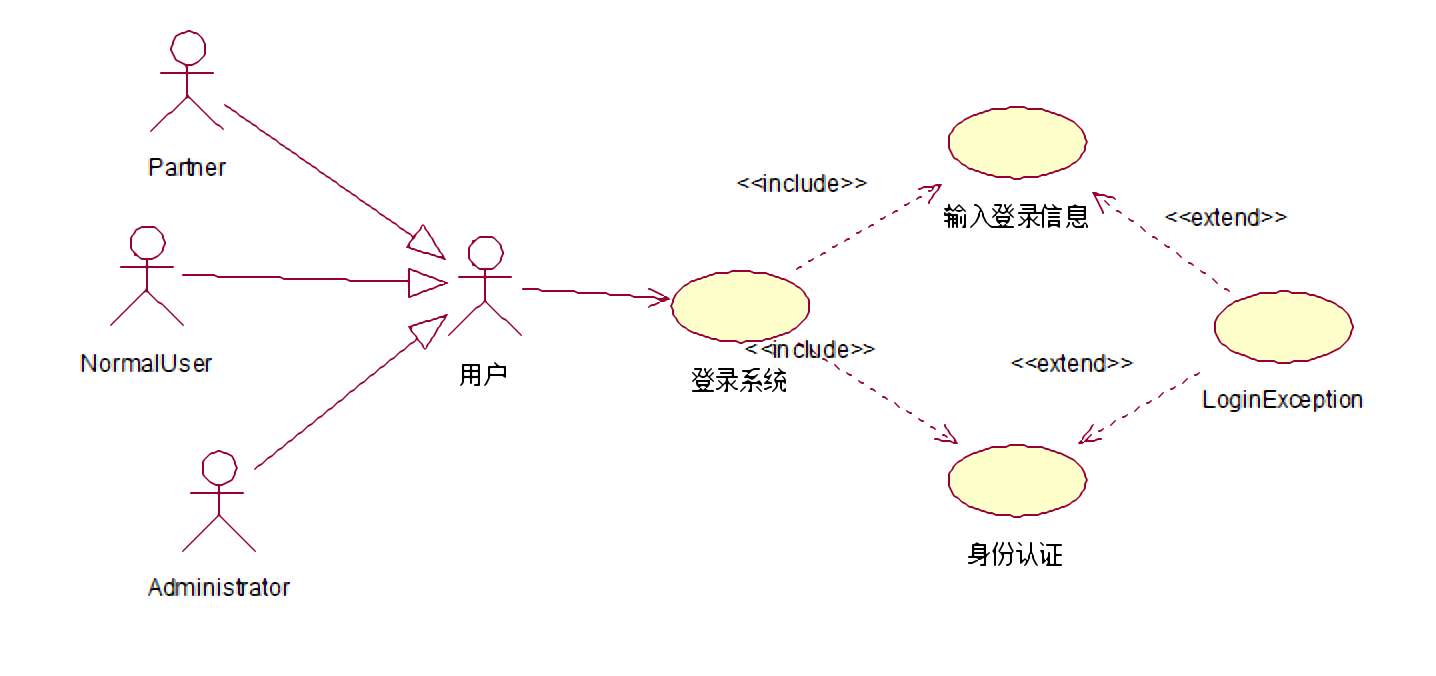
\includegraphics[scale=0.42]{登录_用例图.png}
			\end{center}

			类图: 
			\begin{center}
			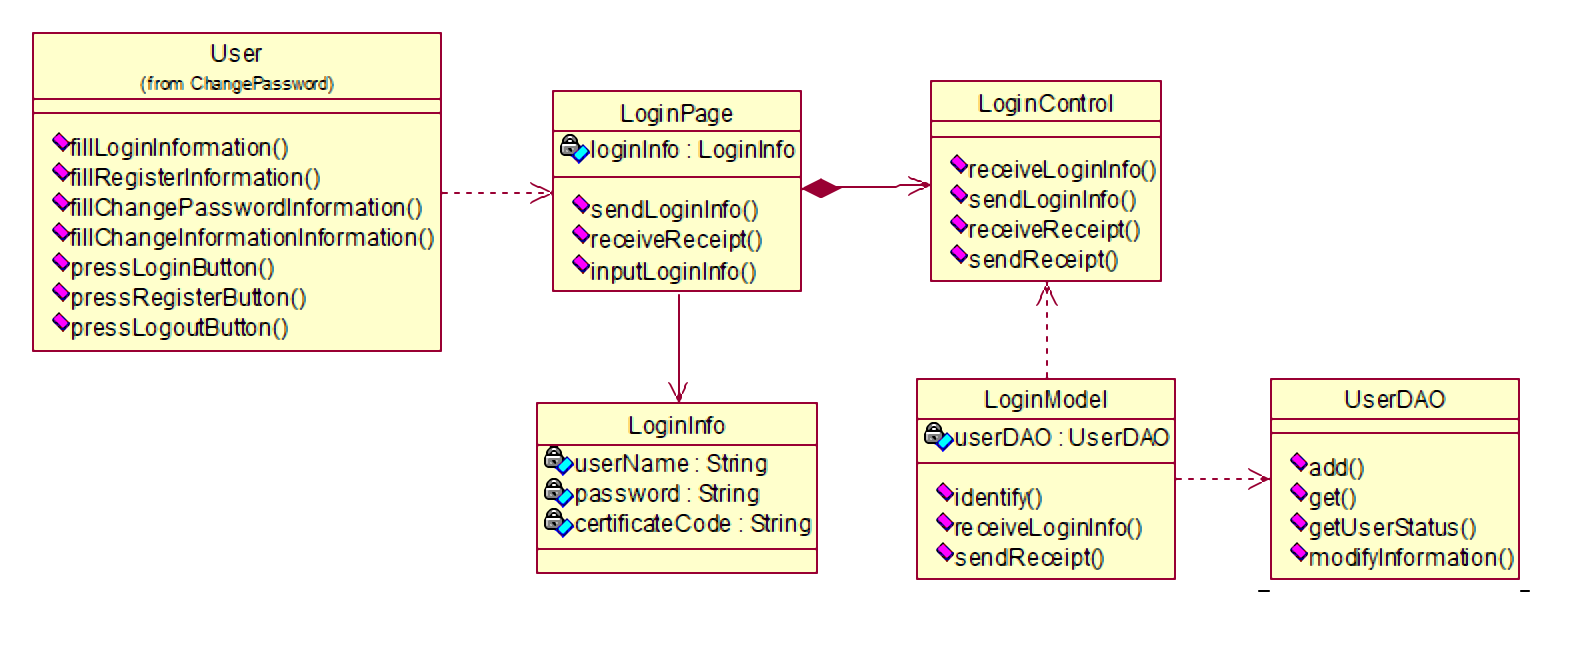
\includegraphics[scale=0.42]{登录_类图.png}
			\end{center}

			状态图: 
			\begin{center}
			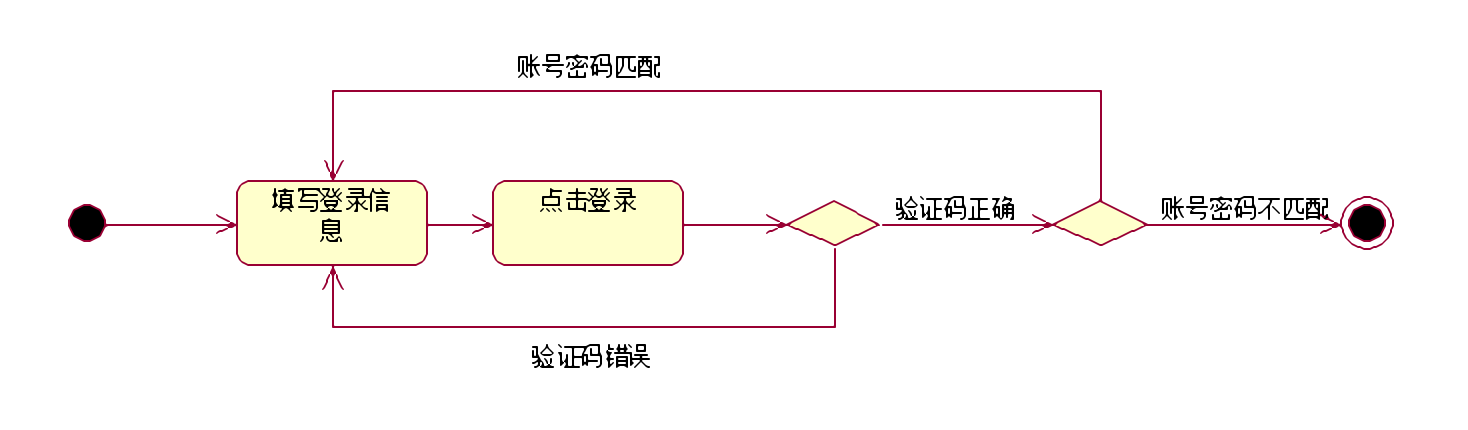
\includegraphics[scale=0.42]{登录_状态图.png}
			\end{center}

			顺序图: 
			\begin{center}
			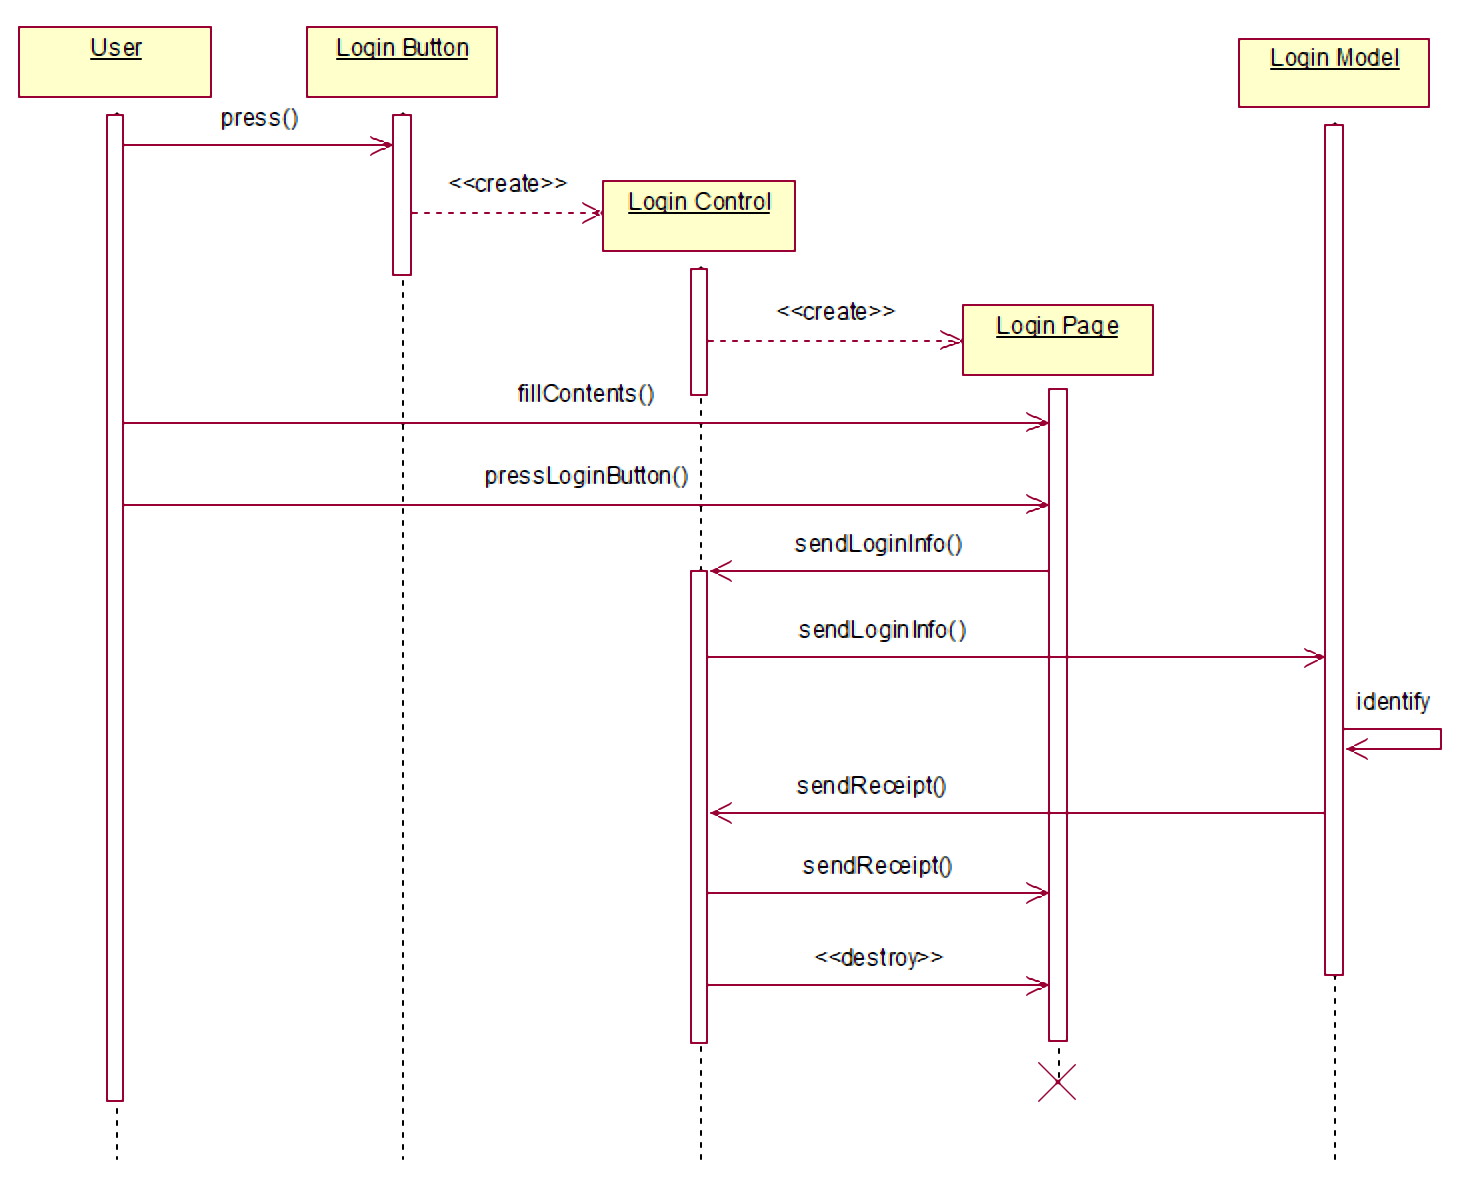
\includegraphics[scale=0.42]{登录_顺序图.png}
			\end{center}

		
		\subsubsection{登出}
			用例: \\ \\
			\begin{tabular}{c|l}
			\hline
			用例名称 & 登出 logout \\ \hline
			参与者 & 酒店合作伙伴Partner, 管理员Administrator, 以及顾客User  \\ \hline
			入口条件 & 用户点击退出按钮 \\ \hline
			事件流 & 	\parbox{33em}{\ \\
						1. 用户点击退出按钮 \\
						2. 系统弹出确认退出窗口 \\
						3. 用户在窗口中点击确认  \\
						4. 系统在后台退出用户的登录状态 \\
						5. 退出成功 \\
						} \\ \hline
			出口条件 & 退出成功 \\ \hline
			质量需求 & \parbox{33em}{\ \\
						用户在确认退出窗口中点击确认 \\
						} \\ \hline
			\end{tabular}\\ \\ \\
			\texttt{
			Algorithm Logout \\
			Input : username \\
			Output : null \\
			1. find the same username in database \\
			2. change the user state to offline \\
			} \\
			
			语言成分分析:
			\begin{center}
			\begin{tabular}{|c|c|c|}
			\hline
			语言成分 & 模型构件 & 实例\\ \hline
			专有名词 & Object & Jack  \\ \hline
			普通名词 & Class & 用户,界面 \\ \hline
			Doing 动词 & Method &  修改,退出 \\ \hline
			Having 动词 & aggregation & 包括 \\ \hline
			形容词, 名词 & Attribute & 用户名 \\ \hline
			\end{tabular}
			\end{center}
			
			用例图: 
			\begin{center}
			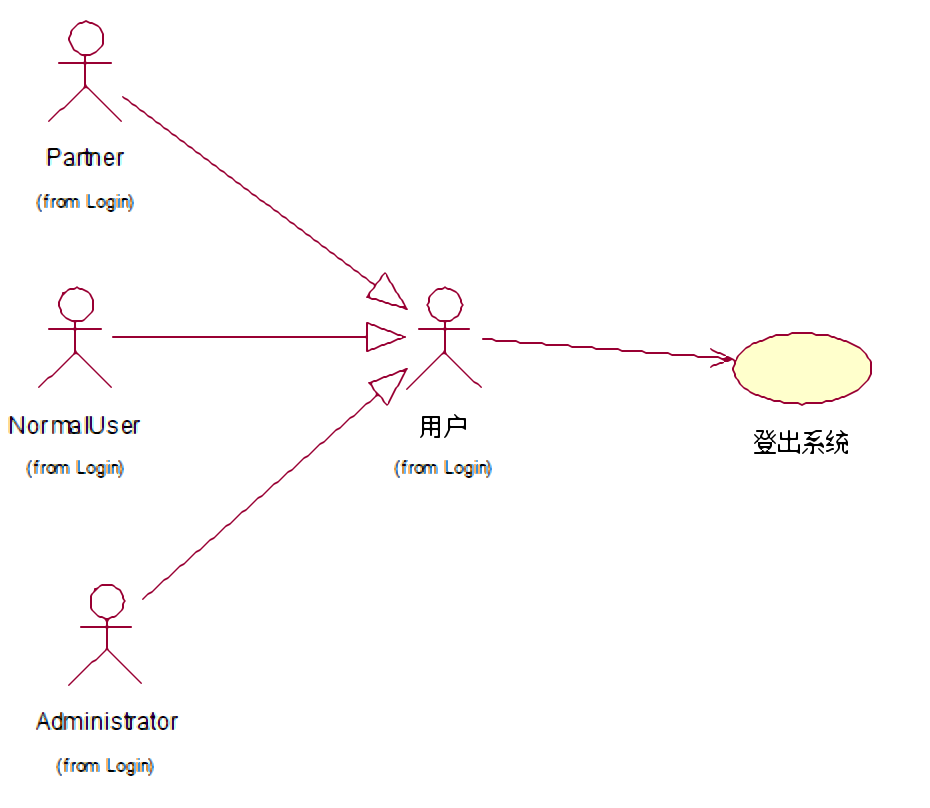
\includegraphics[scale=0.42]{登出_用例图.png}
			\end{center}

			类图: 
			\begin{center}
			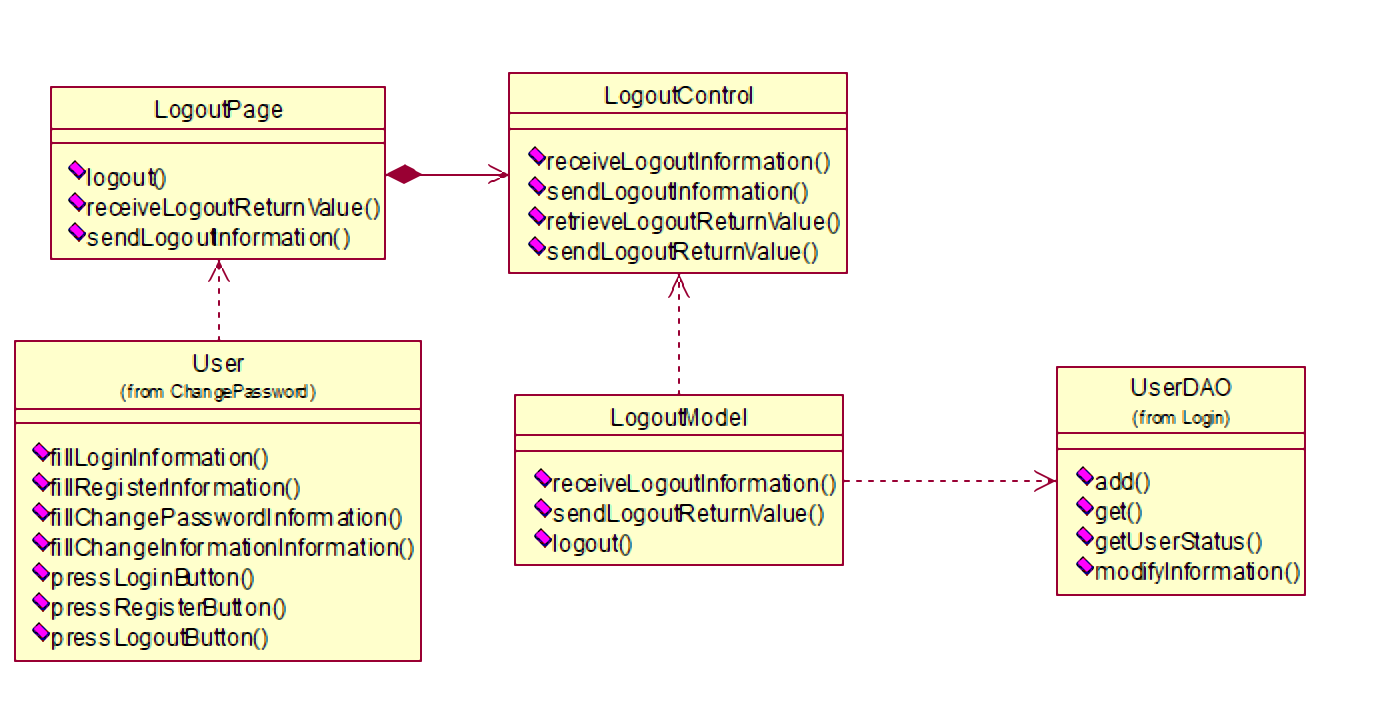
\includegraphics[scale=0.42]{登出_类图.png}
			\end{center}

			状态图: 
			\begin{center}
			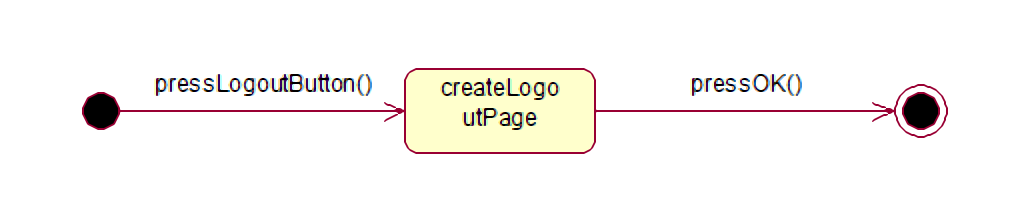
\includegraphics[scale=0.42]{登出_状态图.png}
			\end{center}

			顺序图: 
			\begin{center}
			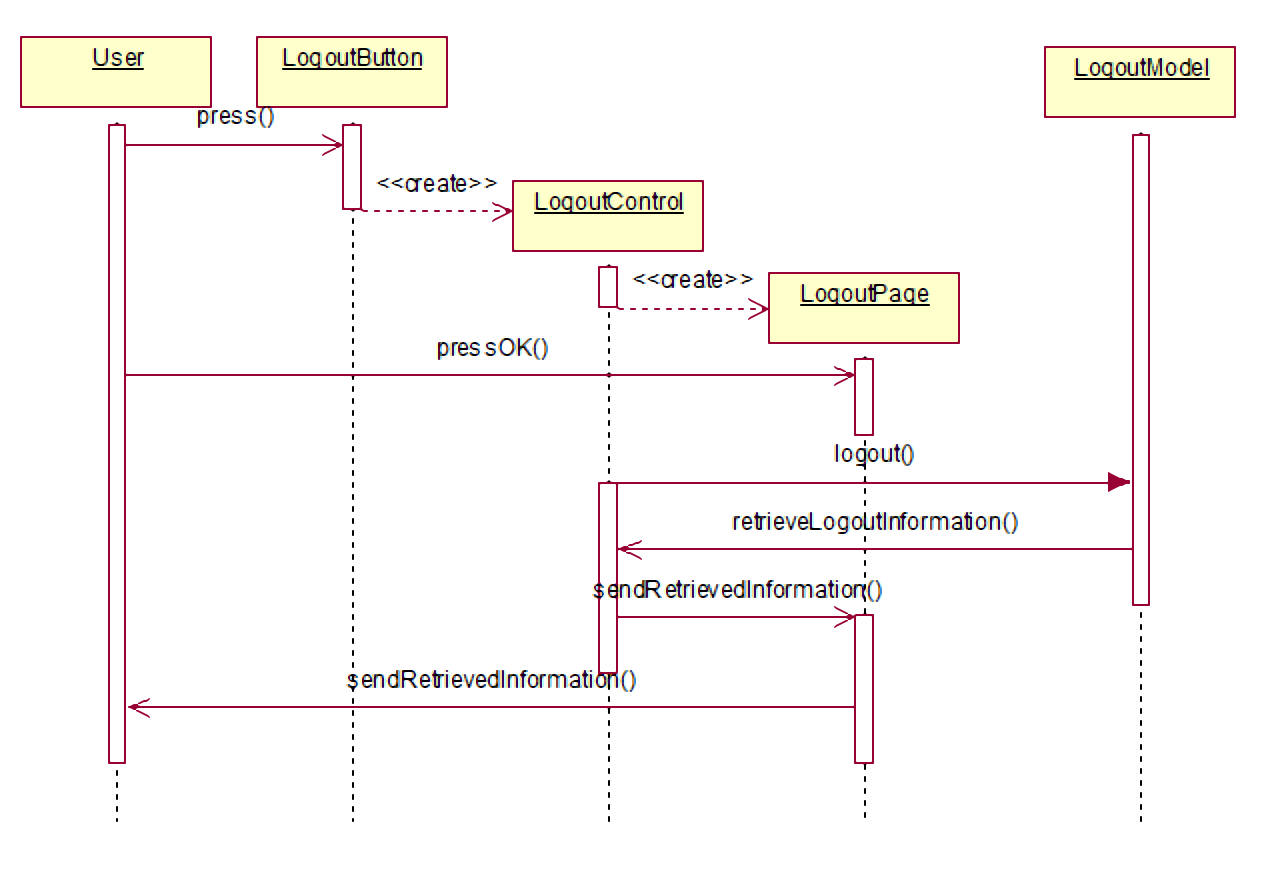
\includegraphics[scale=0.42]{登出_顺序图.png}
			\end{center}
			
		\subsubsection{密码修改}
			用例: \\ \\
			\begin{tabular}{c|l}
			\hline
			用例名称 & 密码修改 Change Password \\ \hline
			参与者 & 酒店合作伙伴Partner, 管理员Administrator, 以及顾客User  \\ \hline
			入口条件 & 用户点击修改密码按钮 \\ \hline
			事件流 & 	\parbox{33em}{\ \\
						1. 用户点击修改密码按钮 \\
						2. 系统弹出修改密码页面, 页面中包含: 新密码, 新密码确认, 验证码, 获取验证码的按钮, 确认按钮以及取消按钮\\
						3. 用户在页面中输入相关信息, 点击确认  \\
						4. 系统判断两次输入密码是否一致, 验证码是否正确 \\
						5. 密码修改成功 \\
						} \\ \hline
			出口条件 & 密码修改成功 \\ \hline
			质量需求 & \parbox{33em}{\ \\
						1. 用户两次输入的密码一致 \\
						2. 用户输入的验证码正确 \\
						} \\ \hline
			\end{tabular}\\ \\ \\
			\texttt{
			Algorithm Change Password \\
			Input : username, password, verifyCode \\
			Output : true or false \\
			1. find the same username in database \\
			2. if(verifyCode is correct) \\
			3.     change the password corresponding to user \\
			4.     return true \\
			5. return false \\
			} \\
			
			语言成分分析:
			\begin{center}
			\begin{tabular}{|c|c|c|}
			\hline
			语言成分 & 模型构件 & 实例\\ \hline
			专有名词 & Object & Jack  \\ \hline
			普通名词 & Class & 用户,界面 \\ \hline
			Doing 动词 & Method &  修改 \\ \hline
			Having 动词 & aggregation & 包括 \\ \hline
			形容词, 名词 & Attribute & 用户名,密码,验证码 \\ \hline
			\end{tabular}
			\end{center}
			
			用例图: 
			\begin{center}
			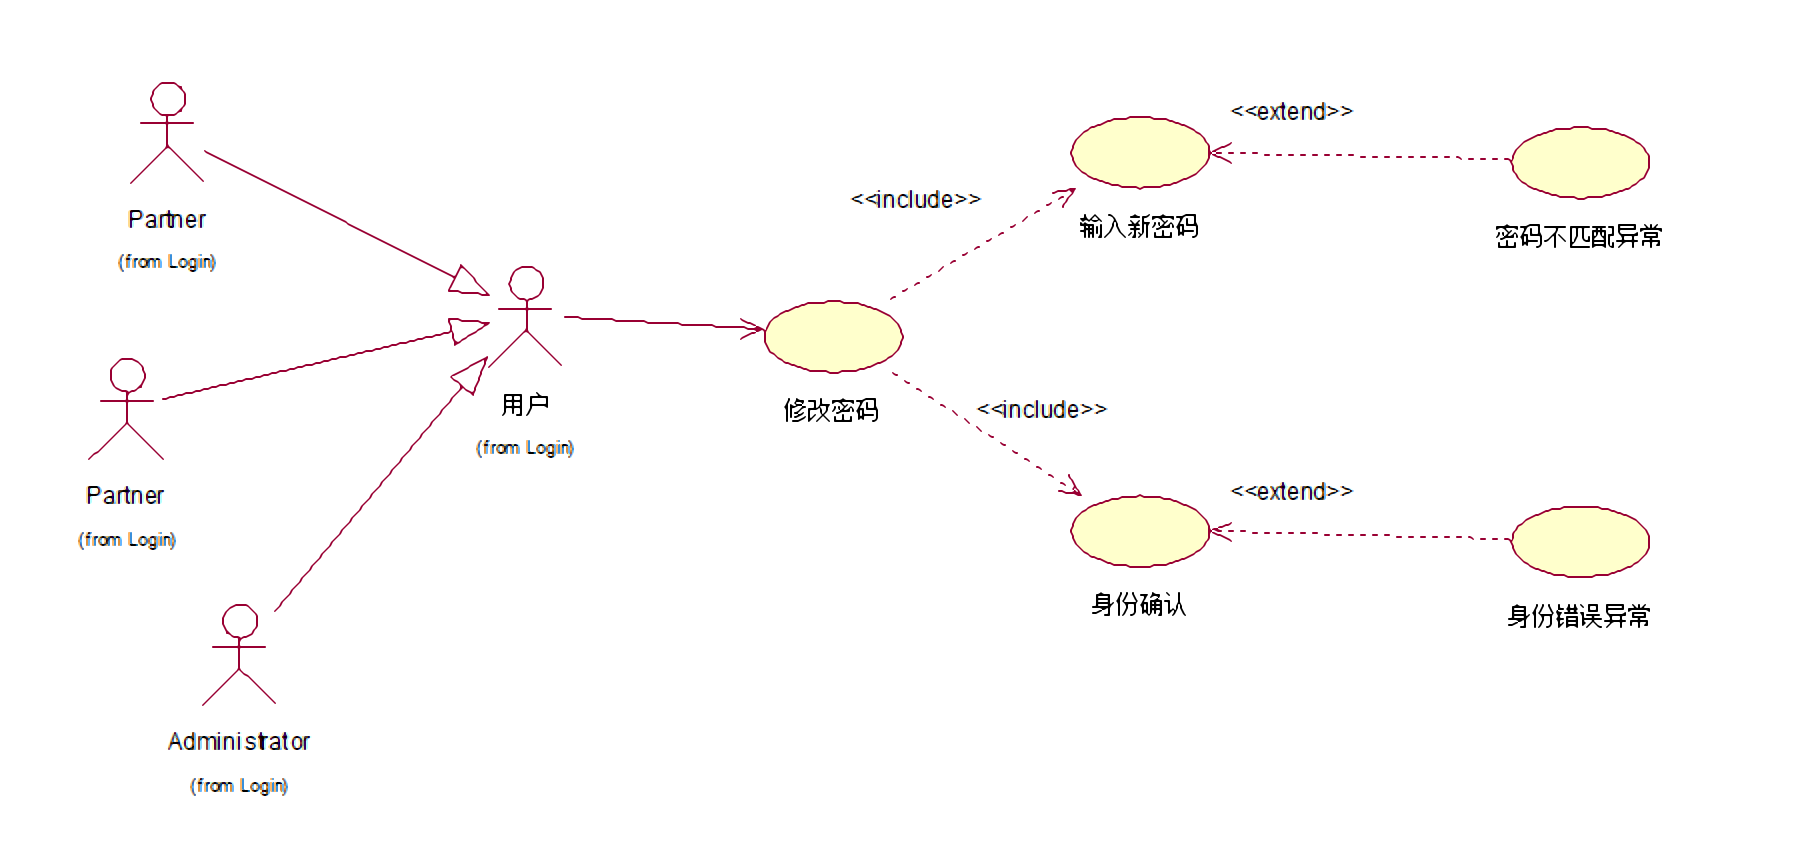
\includegraphics[scale=0.42]{修改密码_用例图.png}
			\end{center}

			类图: 
			\begin{center}
			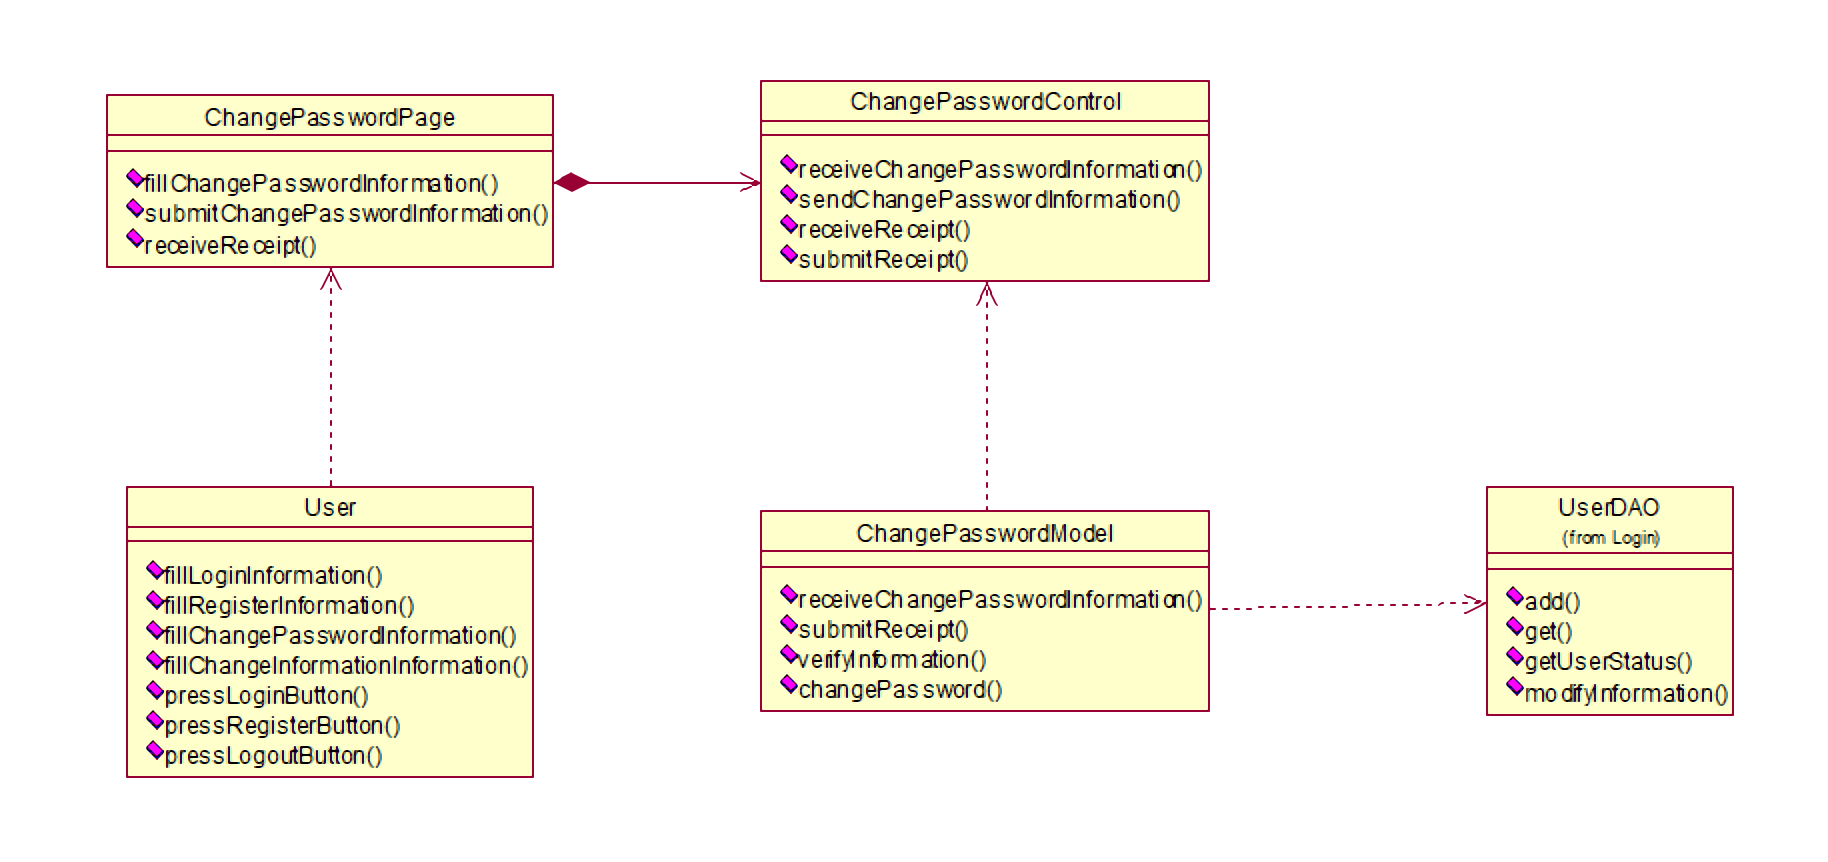
\includegraphics[scale=0.42]{修改密码_类图.png}
			\end{center}

			状态图: 
			\begin{center}
			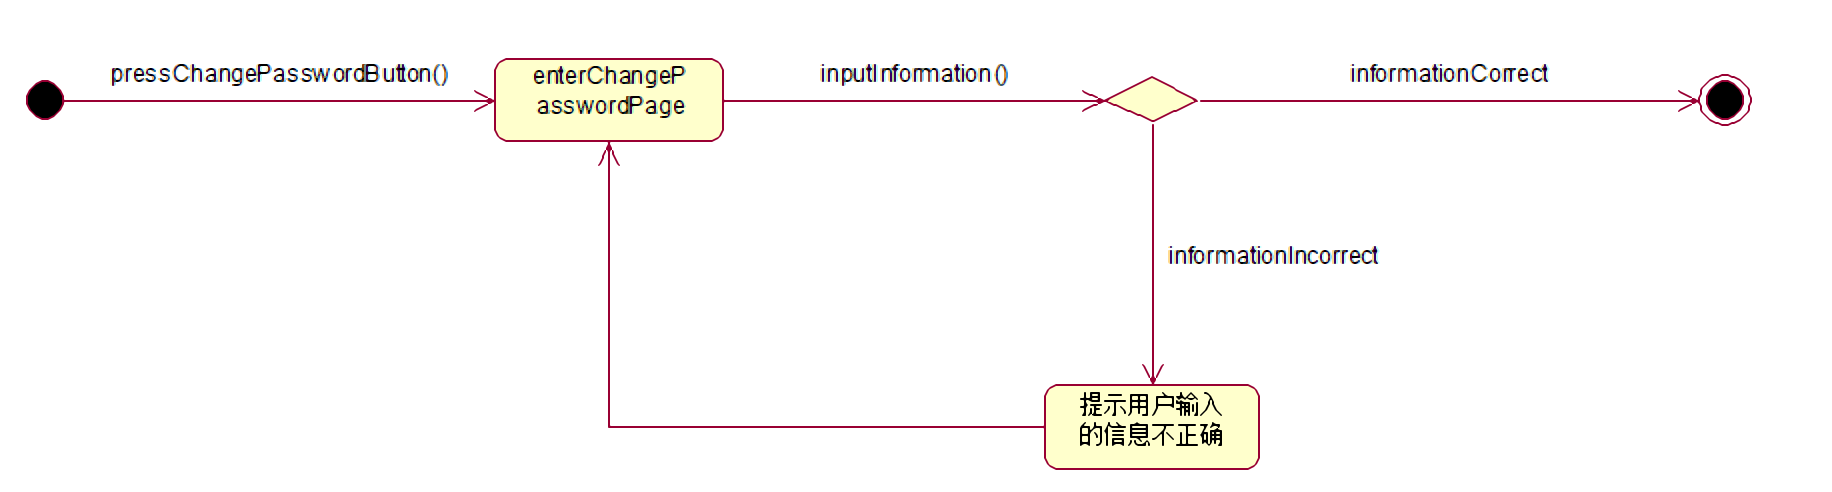
\includegraphics[scale=0.42]{修改密码_状态图.png}
			\end{center}

			顺序图: 
			\begin{center}
			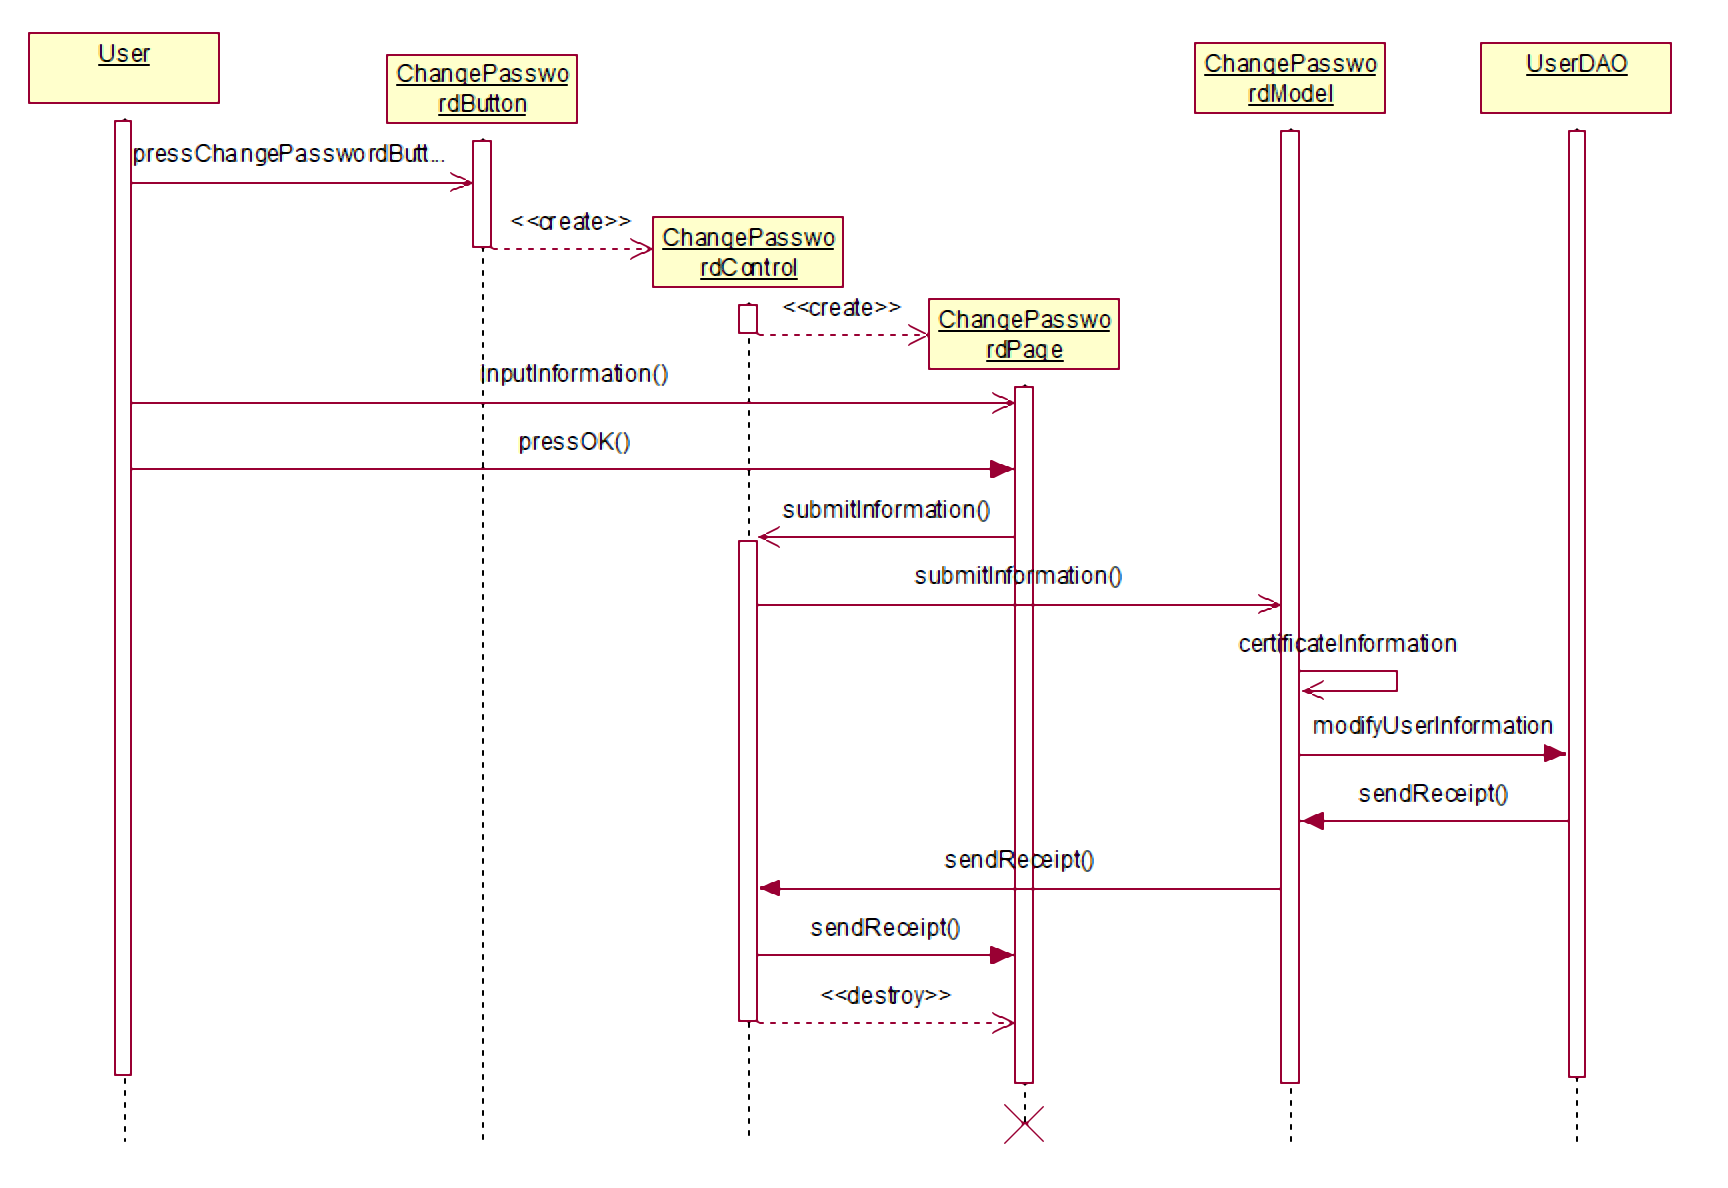
\includegraphics[scale=0.42]{修改密码_顺序图.png}
			\end{center}


		\subsubsection{用户信息修改}
			用例: \\ \\
			\begin{tabular}{c|l}
			\hline
			用例名称 & 用户信息修改 Change Information \\ \hline
			参与者 & 酒店合作伙伴Partner, 管理员Administrator, 以及顾客User  \\ \hline
			入口条件 & 用户点击修改用户信息按钮 \\ \hline
			事件流 & 	\parbox{33em}{\ \\
						1. 用户点击修改用户信息按钮 \\
						2. 系统弹出修改用户信息页面, 页面中包含: 用户名, 手机号, 邮箱, , 验证码, 获取验证码的按钮, 确认按钮以及取消按钮\\
						3. 用户在页面中输入相关信息, 点击确认  \\
						4. 系统判断新手机号和邮箱是否合法, 验证码是否正确 \\
						5. 密码修改成功 \\
						} \\ \hline
			出口条件 & 用户信息修改成功 \\ \hline
			质量需求 & \parbox{33em}{\ \\
						1. 用户输入的手机号和邮箱合法 \\
						2. 用户输入的验证码正确 \\
						} \\ \hline
			\end{tabular}\\ \\ \\
			\texttt{
			Algorithm Change Information \\
			Input : username, verifyCode, userInfo \\
			Output : true or false \\
			1. find the same username in database \\
			2. if(verifyCode is correct) \\
			3.     change the userInfo corresponding to user \\
			4.     return true \\
			5. return false \\
			} \\
			
			语言成分分析:
			\begin{center}
			\begin{tabular}{|c|c|c|}
			\hline
			语言成分 & 模型构件 & 实例\\ \hline
			专有名词 & Object & Jack  \\ \hline
			普通名词 & Class & 用户,界面 \\ \hline
			Doing 动词 & Method &  修改 \\ \hline
			Having 动词 & aggregation & 包括 \\ \hline
			形容词, 名词 & Attribute & 用户名,用户信息,验证码 \\ \hline
			\end{tabular}
			\end{center}
			
			用例图: 
			\begin{center}
			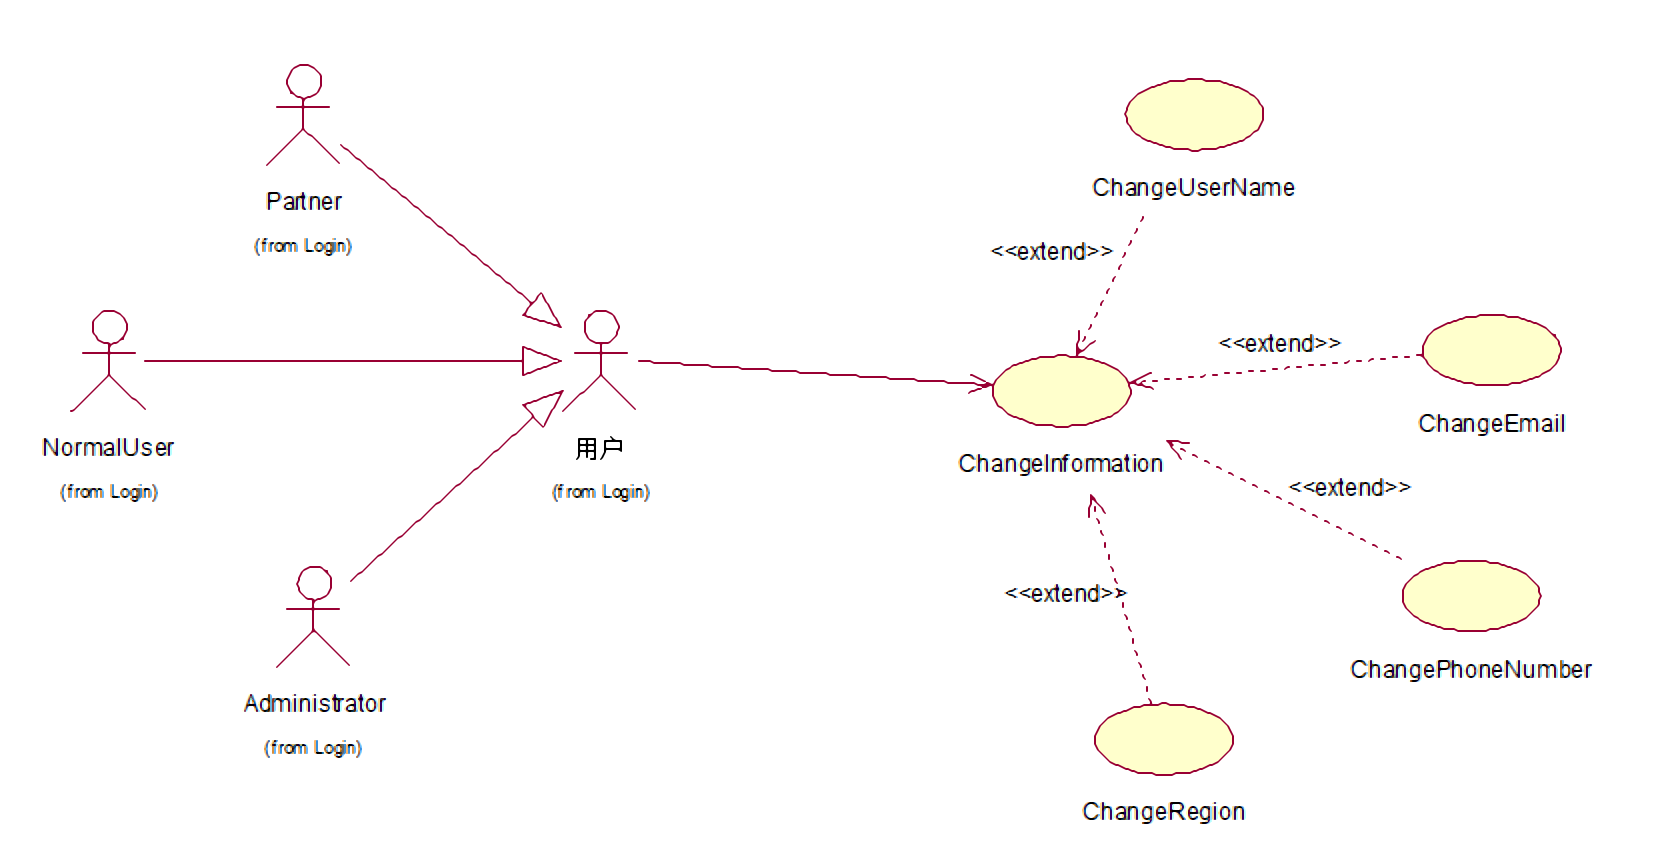
\includegraphics[scale=0.42]{修改用户信息_用例图.png}
			\end{center}

			类图: 
			\begin{center}
			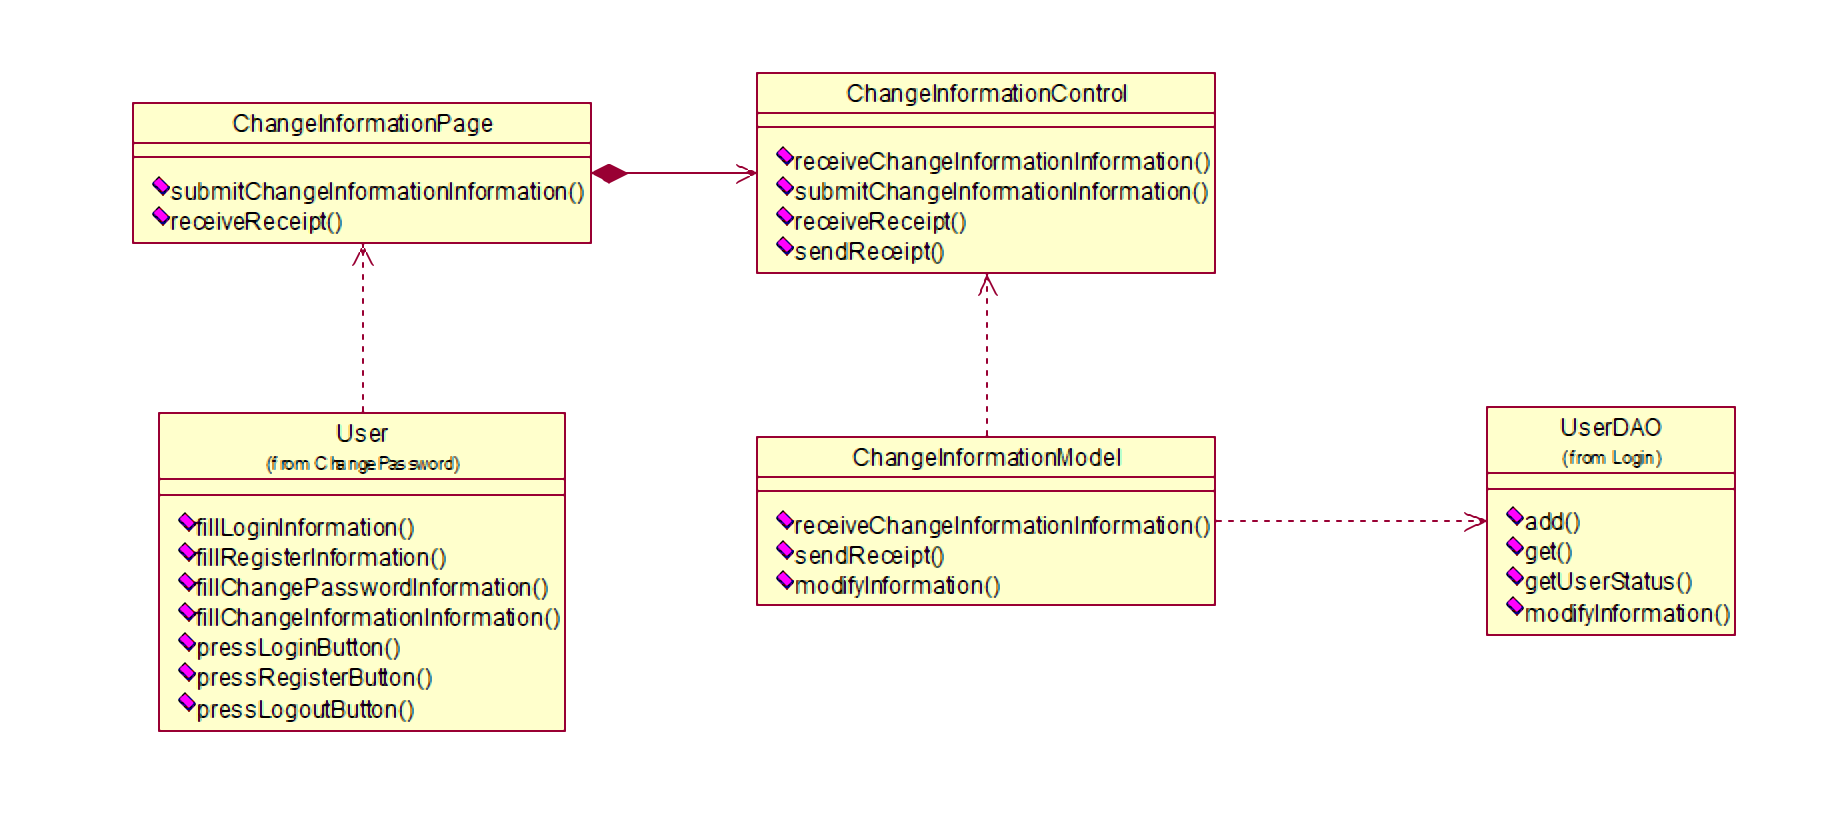
\includegraphics[scale=0.42]{修改用户信息_类图.png}
			\end{center}

			状态图: 
			\begin{center}
			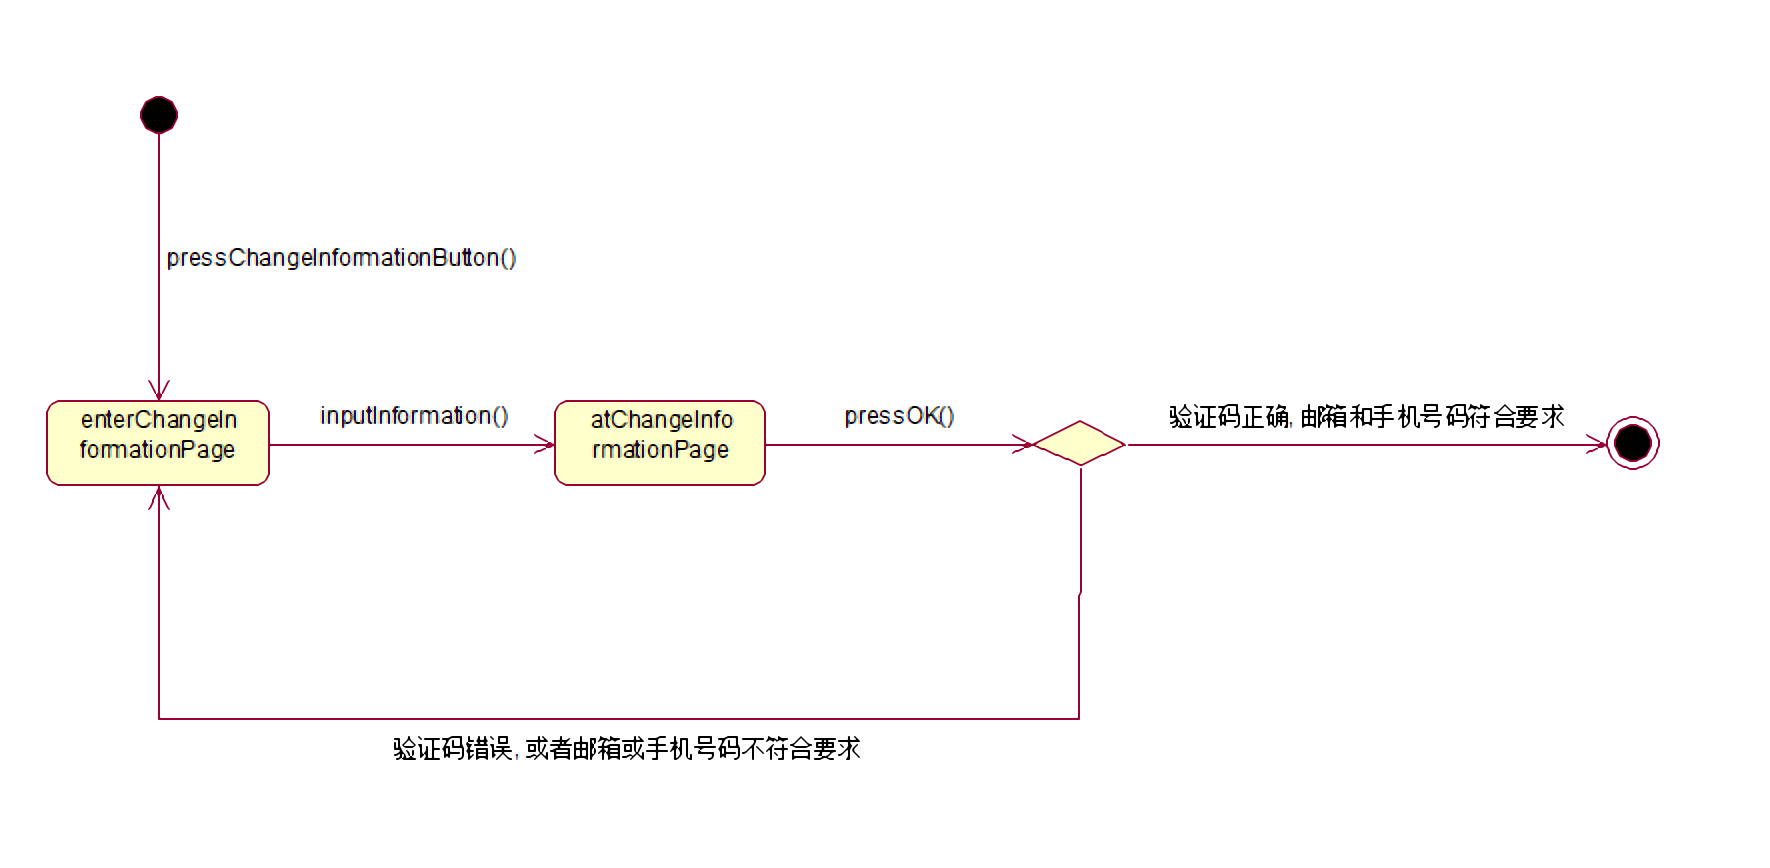
\includegraphics[scale=0.42]{修改用户信息_状态图.png}
			\end{center}

			顺序图: 
			\begin{center}
			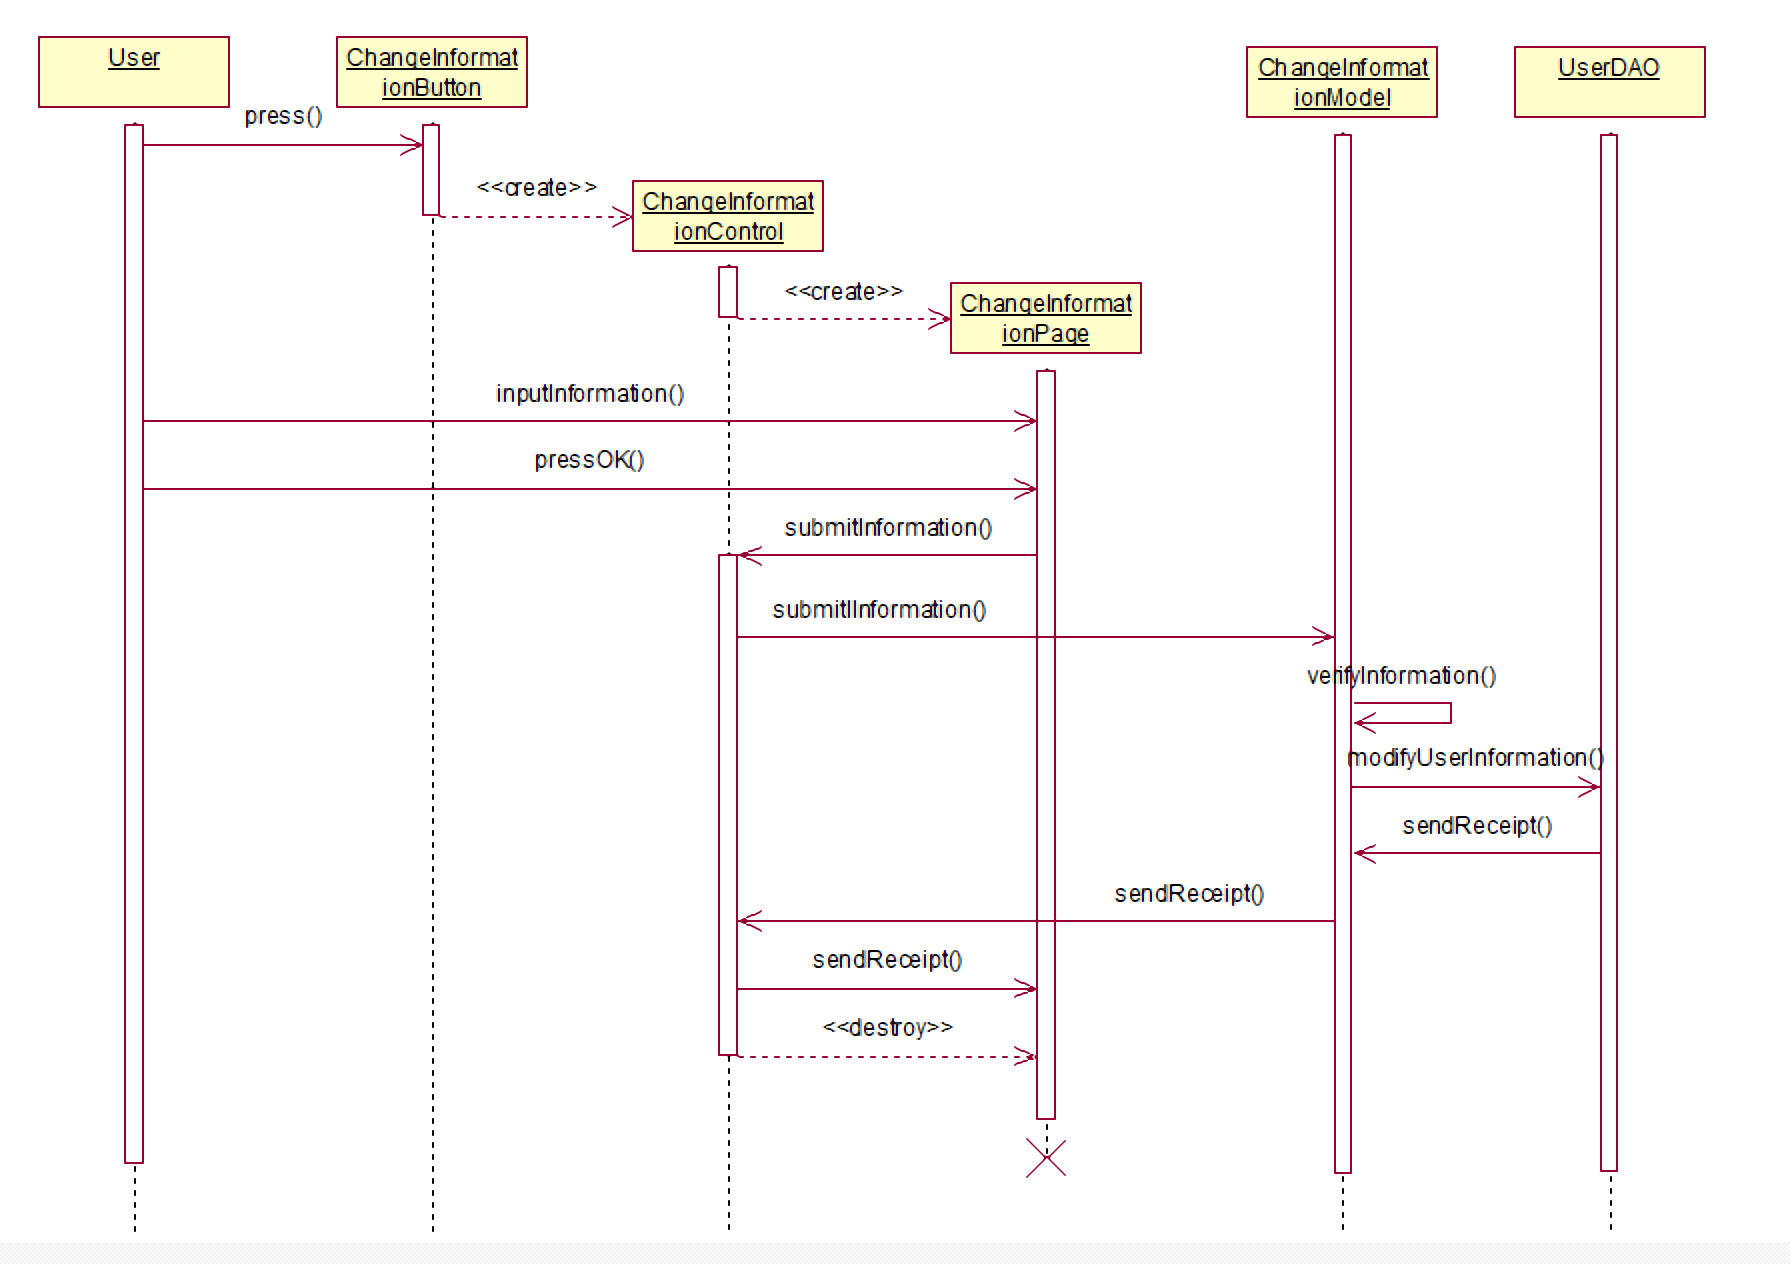
\includegraphics[scale=0.42]{修改用户信息_顺序图.png}
			\end{center}
			
			
			
			
	\subsection{酒店合作伙伴Partner}
		\subsubsection{管理酒店信息}
		\subsubsection{查看或回复评论}
		\subsubsection{联系客服}
		\subsubsection{退出加盟}
		
	\subsection{管理员Administrator}
		\subsubsection{管理加盟申请}
		\subsubsection{管理用户}
		
		
	
	\subsection{普通用户User}
	
		\subsubsection{酒店搜索}
			用例: \\ \\
			\begin{tabular}{c|l}
			\hline
			用例名称 & 酒店搜索 Hotel Search \\ \hline
			参与者 & 顾客User  \\ \hline
			入口条件 & 用户在搜索界面上输入相关信息, 点击搜索按钮 \\ \hline
			事件流 & 	\parbox{33em}{\ \\
						1. 用户在搜索界面上输入城市, 入住日期,  离开日期, 点击搜索按钮 \\
						2. 系统获取用户的输入信息, 在数据库中查找符合条件的酒店 \\
						3. 系统将符合条件的酒店显示到界面上, 并在地图上标注  \\
						} \\ \hline
			出口条件 & 系统显示搜索结果或用户主动退出 \\ \hline
			质量需求 & \parbox{33em}{\ \\
						用户输入的搜索信息完整 \\
						} \\ \hline
			\end{tabular}

		\subsubsection{预订}
		\subsubsection{支付}
		\subsubsection{评论}
		\subsubsection{收藏}
		\subsubsection{订单查询}
		\subsubsection{添加信用卡}
			用例: \\ \\
			\begin{tabular}{c|l}
			\hline
			用例名称 & 添加信用卡 Add\ CreditCard \\ \hline
			参与者 & 用户 User  \\ \hline
			入口条件 & 用户 User 点击添加信用卡按钮 \\ \hline
			事件流 & 	\parbox{33em}{\ \\
						1. 用户 User 点击添加信用卡按钮 \\
						2. Booking系统弹出添加信用卡页面 \\
						3. 用户补充相关信息, 点击提交按钮或者取消按钮  \\
						4. 若用户点击提交, Booking 系统检查信用卡是否有效, 若有效, 保存相关信息, 若无效, 显示错误提示, 若用户选择取消则直接返回设置界面 \\
						} \\ \hline
			出口条件 & \parbox{33em}{\ \\
						提交成功或者点击取消按钮 \\
						} \\ \hline
			质量需求 & \parbox{33em}{\ \\
						1. 网络通畅 \\
						2. 当前用户处于登录状态 \\
						} \\ \hline
			\end{tabular} \\ \\ \\
			\texttt{
			Algorithm AddCreditCard \\
			Input : cardNumber, password \\
			Output : true or false \\
			1.Search the dataset to check if the credit Card valid \\
			2.if true \\
			3.  save the credit card information. \\
			4.	return true \\
			5.else \\
			6.  return false \\
			} \\
			
			语言成分分析:
			\begin{center}
			\begin{tabular}{|c|c|c|}
			\hline
			语言成分 & 模型构件 & 实例\\ \hline
			专有名词 & Object & GDW  \\ \hline
			普通名词 & Class & 用户, 界面 \\ \hline
			Doing 动词 & Method &  显示, 修改, 检查, 保存 \\ \hline
			Being 动词 & inheritance & 是……的某一项 \\ \hline
			Having 动词 & aggregation &  包括 \\ \hline
			情态动词 & constraint & 必须 \\ \hline
			形容词, 名词 & Attribute & 货币类型 \\ \hline
			\end{tabular}
			\end{center}
			
			类图: 
			\begin{center}
			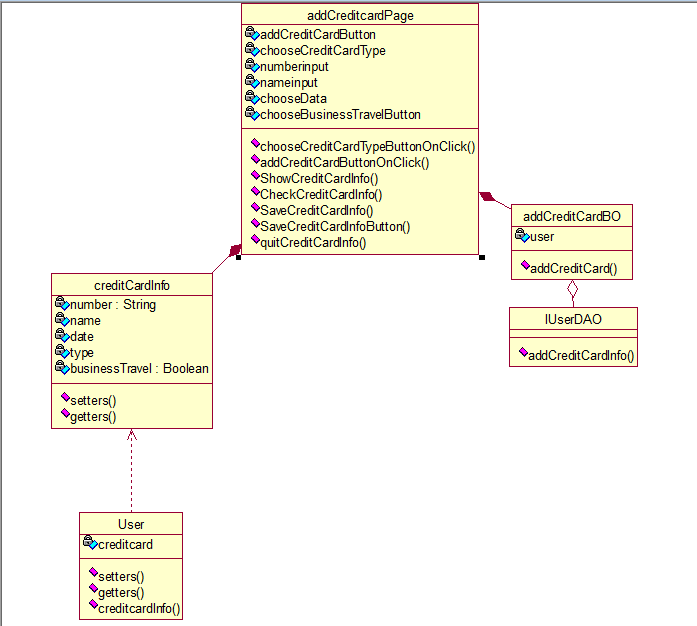
\includegraphics[scale=0.42]{普通用户添加信用卡类图.png}
			\end{center}

			状态图: 
			\begin{center}
			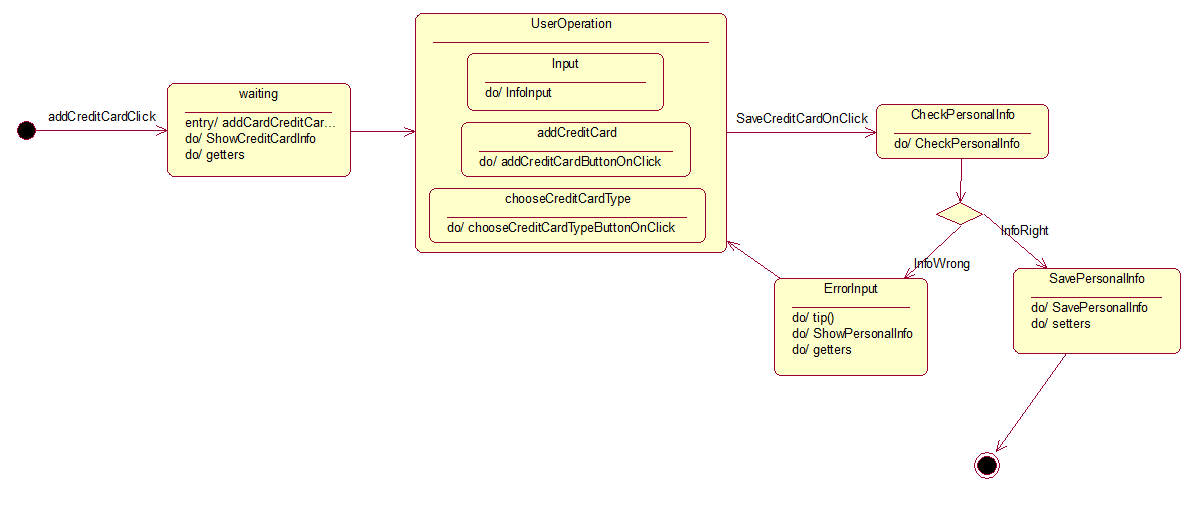
\includegraphics[scale=0.42]{普通用户添加信用卡状态图.png}
			\end{center}

			顺序图: 
			\begin{center}
			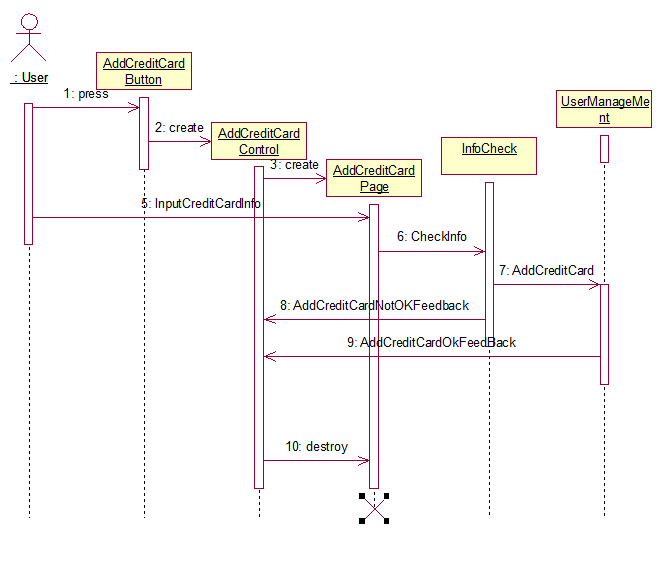
\includegraphics[scale=0.42]{普通用户添加信用卡顺序图.png}
			\end{center}
	
	\subsection{其他功能}
		\subsubsection{查看常见问题和解答}
			用例: \\ \\
			\begin{tabular}{c|l}
			\hline
			用例名称 & 查看常见问题和解答 \\ \hline
			参与者 & 顾客User  \\ \hline
			入口条件 & 顾客 User 选择常见问题及解答 \\ \hline
			事件流 & 	\parbox{33em}{\ \\
						1. 用户在搜索界面上输入城市, 入住日期,  离开日期, 点击搜索按钮 \\
						2. 系统获取用户的输入信息, 在数据库中查找符合条件的酒店 \\
						3. 系统将符合条件的酒店显示到界面上, 并在地图上标注  \\
						} \\ \hline
			出口条件 & \parbox{33em}{\ \\
						1. 顾客User得到满意答案 \\
						2.  	顾客User进一步选择联系客服,修改订单,取消订单等选项 \\
						} \\ \hline
			质量需求 & \parbox{33em}{\ \\
						网络通畅,有足够多的问题种类及回答,答案质量高 \\
						} \\ \hline
			\end{tabular} \\ \\ \\
			\texttt{
			Algorithm Answers \\
				Input:null \\
				Output: answers \\
				1.	click Customer service \\
				2.	jump to inquiry page \\
				3.	return null \\
			} \\
			\texttt{
			Algorithm SearchByKeyword \\
			Input:Keywords \\
			Output:answers \\
			1.	search the database with the keyword \\
			2.	if searched \\
			3.	show the related issues and the answers \\
			4.	else keep the page \\
			5.	return null \\
			} \\

			语言成分分析: \\
			\begin{center}
			\begin{tabular}{|c|c|c|}
			\hline
			语言成分 & 模型构件 & 实例\\ \hline
			专有名词 & Object & Rose  \\ \hline
			普通名词 & Class & 用户, 界面 \\ \hline
			Doing 动词 & Method & 点击, 选择, 进入, 搜索, 输入, 显示 \\ \hline
			名词 & Attribute & 按钮, 链接, 关键词, 结果, 评价 \\ \hline
			\end{tabular}
			\end{center}
			
			类图: 
			\begin{center}
			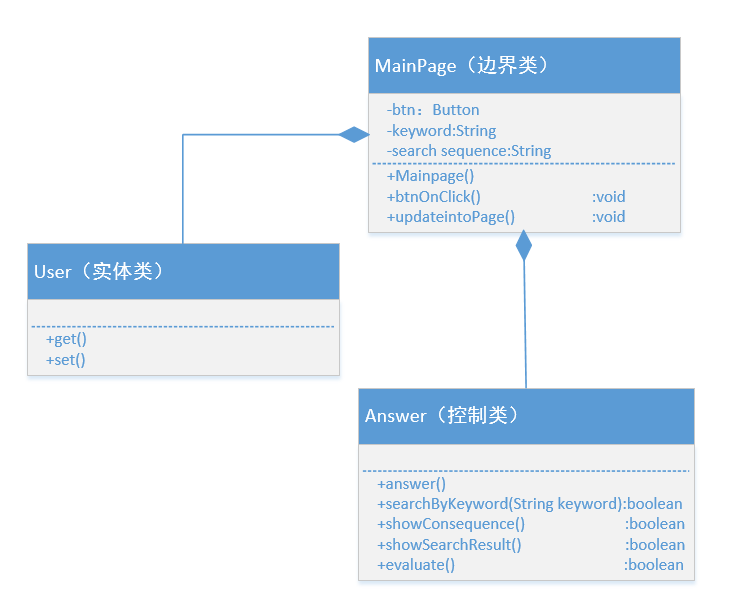
\includegraphics[scale=0.42]{4.1类图.png}
			\end{center}
			
			状态图: 
			\begin{center}
			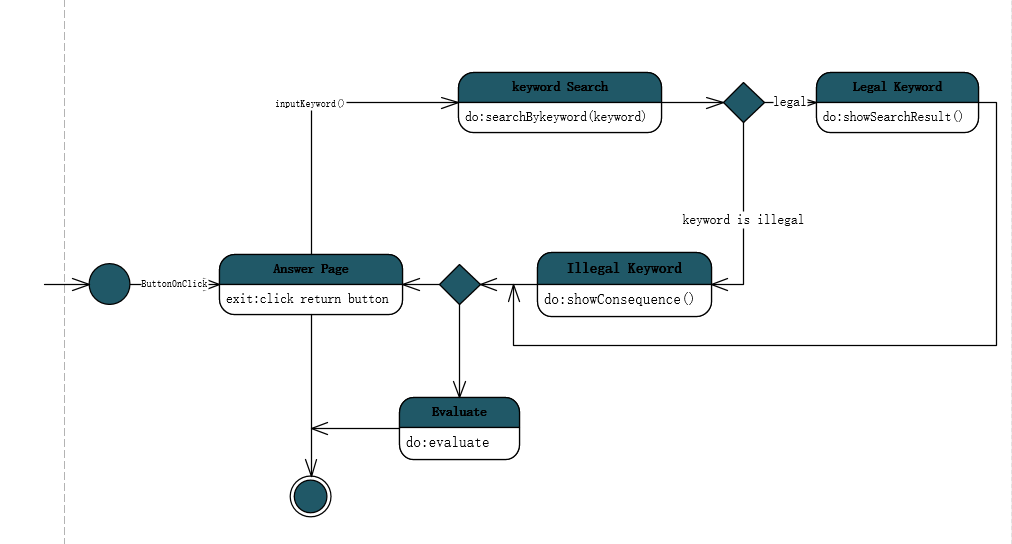
\includegraphics[scale=0.42]{4.1状态图.png}
			\end{center}

			顺序图: 
			\begin{center}
			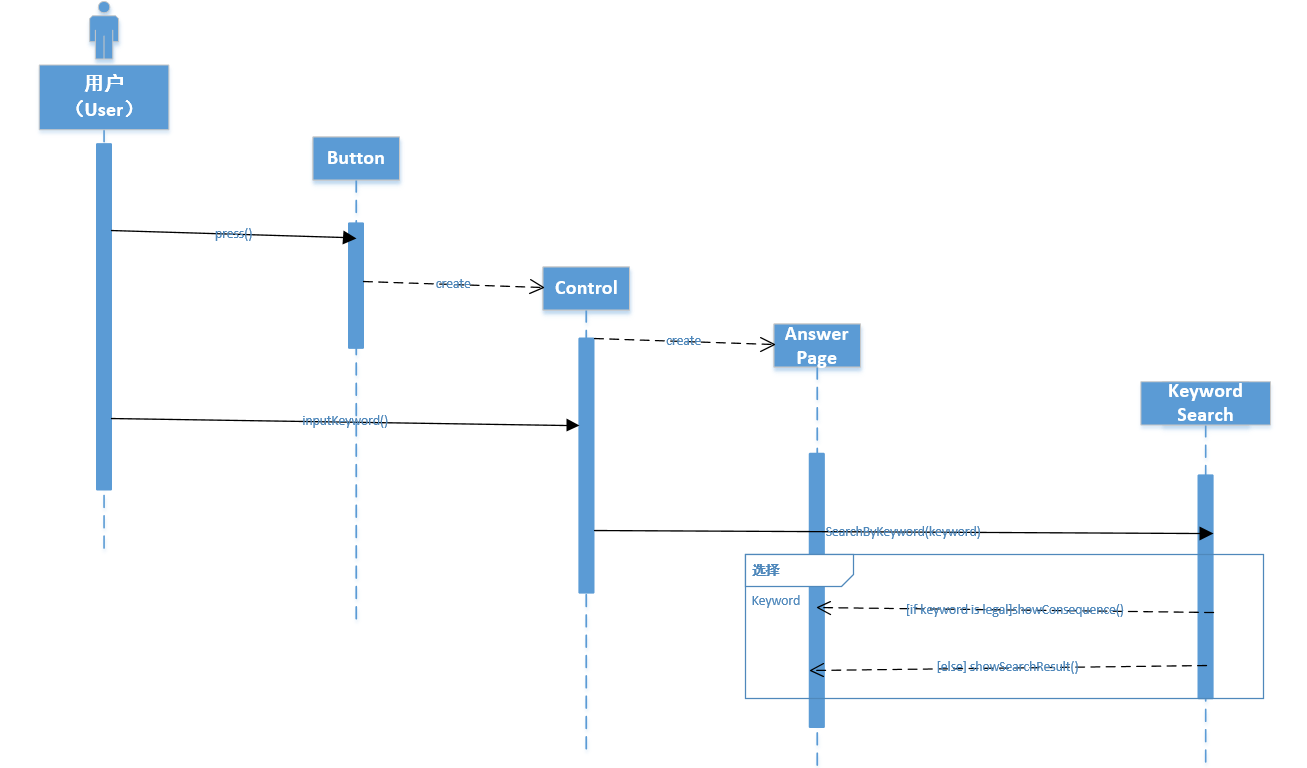
\includegraphics[scale=0.42]{4.1顺序图.png}
			\end{center}

			


		\subsubsection{查看相关条款 Relevant\ Terms}
			用例: \\ \\
			\begin{tabular}{c|l}
			\hline
			用例名称 & 查看相关条款 Relevant\ Terms \\ \hline
			参与者 & 顾客User  \\ \hline
			入口条件 & 顾客 User  点击网站下方的相关条款选项 \\ \hline
			事件流 & 	\parbox{33em}{\ \\
						1. 顾客 User  点击网站下方的相关条款选项 \\
						2. 顾客 User 选择了想要了解的相关条款(如良好行为准则, 条款及条件介绍等) \\
						3. 网站会调到顾客选择的相关部分  \\
						4. 顾客 User 可以选择打印或保存 \\
						} \\ \hline
			出口条件 & \parbox{33em}{\ \\
						显示相关条款内容 \\
						} \\ \hline
			质量需求 & \parbox{33em}{\ \\
						网络通畅 \\
						} \\ \hline
			\end{tabular} \\ \\ \\
			\texttt{
			Algorithm Search Relevant Terms \\
			Input:null \\
			Output:null \\
			1.	jump to Travel terms and conditions page \\
			2.	return null \\
			} \\

			语言成分分析: \\
			\begin{center}
			\begin{tabular}{|c|c|c|}
			\hline
			语言成分 & 模型构件 & 实例\\ \hline
			专有名词 & Object & Rose  \\ \hline
			普通名词 & Class & 用户, 界面 \\ \hline
			Doing 动词 & Method & 点击, 选择, 进入, 显示 \\ \hline
			名词 & Attribute & 按钮 \\ \hline
			\end{tabular}
			\end{center}
			
			类图: 
			\begin{center}
			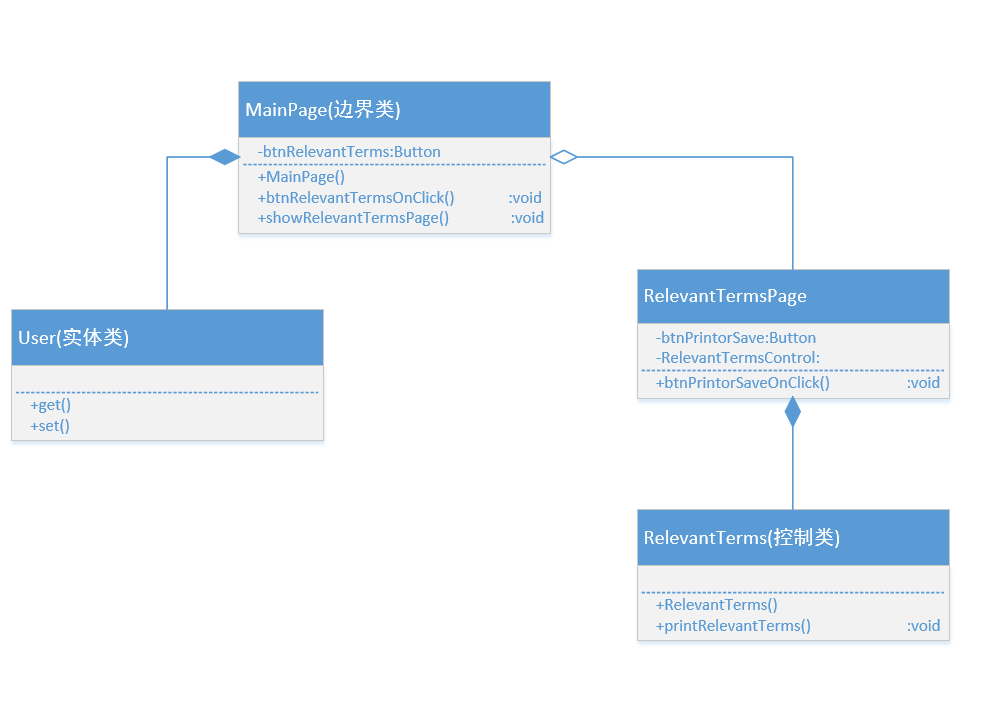
\includegraphics[scale=0.42]{4.2类图.png}
			\end{center}

			状态图: 
			\begin{center}
			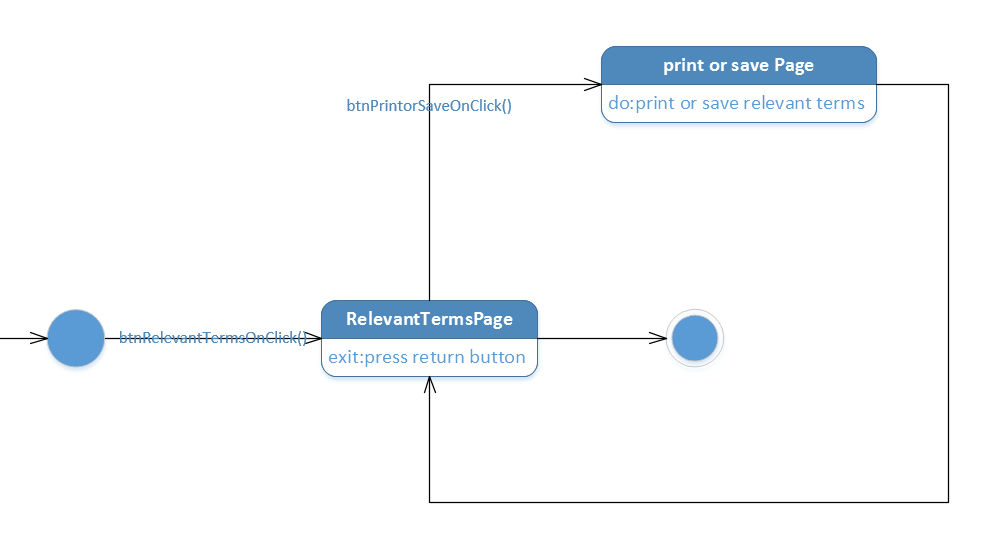
\includegraphics[scale=0.42]{4.2状态图.png}
			\end{center}

			顺序图: 
			\begin{center}
			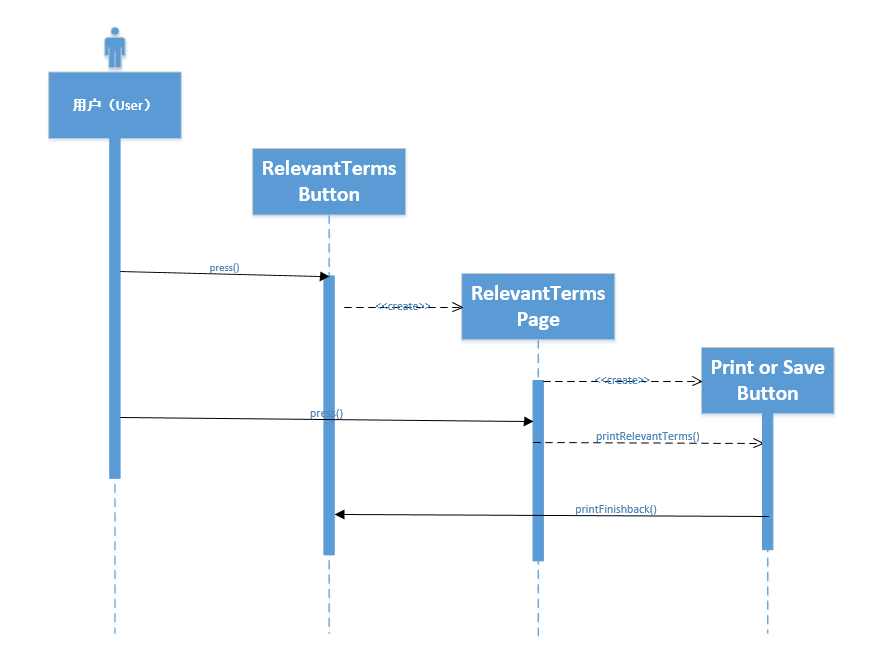
\includegraphics[scale=0.42]{4.2顺序图.png}
			\end{center}



		\subsubsection{咨询客服 Consulting\ service}
			用例: \\ \\
			\begin{tabular}{c|l}
			\hline
			用例名称 & 咨询客服 Consulting\ service \\ \hline
			参与者 & 顾客User  \\ \hline
			入口条件 &  	顾客User点击网站下方的客服帮助选项 \\ \hline
			事件流 & 	\parbox{33em}{\ \\
						1. 顾客User点击网站下方的客服帮助选项 \\
						2. 顾客User点击'拨打电话或发邮件联系我们'的按钮 \\
						3. 顾客User填写预定编号、邮箱、电话、需要解决的问题  \\
						4. 顾客User点击发送按钮  \\
						5. 顾客User也可选择拨打网页下方提供的服务电话  \\
						} \\ \hline
			出口条件 & \parbox{33em}{\ \\
						发送完毕 \\
						} \\ \hline
			质量需求 & \parbox{33em}{\ \\
						网络通畅 \\
						} \\ \hline
			\end{tabular} \\ \\ \\
			\texttt{
			Algorithm Search Relevant Terms \\
			Input:null \\
			Output:null \\
			1.	click Customer service \\
			2.	write phone number,questions \\
			3.	click send button \\
			4.	return null \\
			} \\ \\ \\

			语言成分分析: \\
			\begin{center}
			\begin{tabular}{|c|c|c|}
			\hline
			语言成分 & 模型构件 & 实例\\ \hline
			专有名词 & Object & Rose  \\ \hline
			普通名词 & Class & 用户, 界面 \\ \hline
			Doing 动词 & Method & 点击, 进入, 拨打, 填写, 发送 \\ \hline
			名词 & Attribute & 按钮, 邮箱, 预订编号, 需要解决的问题 \\ \hline
			\end{tabular}
			\end{center}

			类图: 
			\begin{center}
			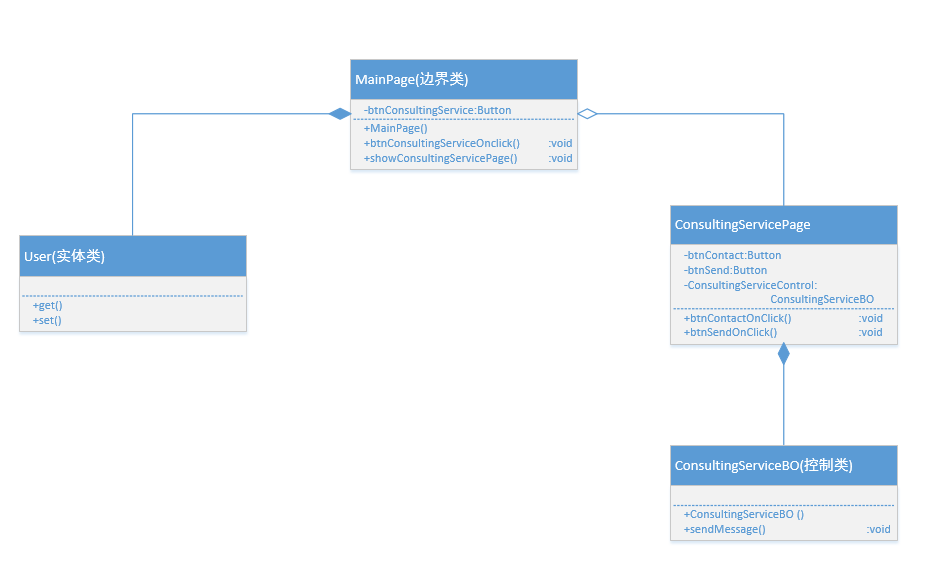
\includegraphics[scale=0.42]{4.3类图.png}
			\end{center}

			状态图: 
			\begin{center}
			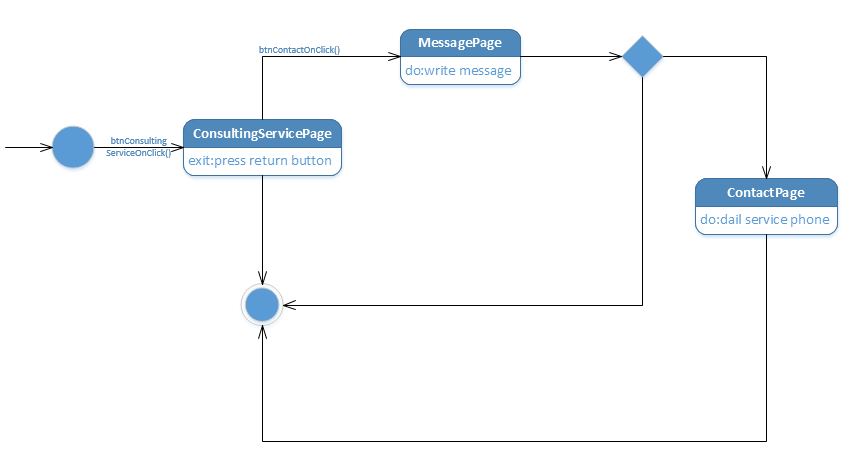
\includegraphics[scale=0.42]{4.3状态图.png}
			\end{center}

			顺序图: 
			\begin{center}
			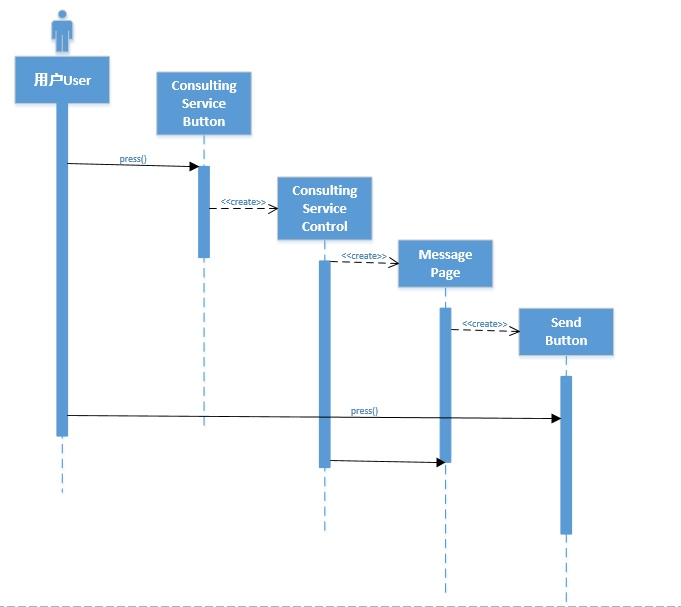
\includegraphics[scale=0.42]{4.3顺序图.png}
			\end{center}


	\subsection{软件设置}
		\subsubsection{语言选择}
			用例: \\ \\
			\begin{tabular}{c|l}
			\hline
			用例名称 & 选择语言 Choose\ Language \\ \hline
			参与者 & 用户 User, 合作伙伴 Partner, 管理员 Administrator  \\ \hline
			入口条件 & 用户 User 点击国旗按钮 \\ \hline
			事件流 & 	\parbox{33em}{\ \\
						1. 用户点击国旗按钮 \\
						2. Booking系统返回语言选择界面 \\
						3. 用户 User 选择需要的语言并点击  \\
						4.  页面刷新, 并更新成相应的语言 \\
						} \\ \hline
			出口条件 & \parbox{33em}{\ \\
						界面语言更换 \\
						} \\ \hline
			质量需求 & \parbox{33em}{\ \\
						网络通畅 \\
						} \\ \hline
			\end{tabular} \\ \\ \\
			\texttt{
			Algorithm ChooseLanguage:\\
			Input: selected language(the language which the user selected), the language set, the set of URLs in different languages \\
			Output: null \\
			1: for each language in the language set do \\
			2:	if current language == selected language \\
			3:		address←URL in selected language \\
			4: end for \\
			5: refresh the page \\
			6: return null \\
			} \\

			语言成分分析: \\
			\begin{center}
			\begin{tabular}{|c|c|c|}
			\hline
			语言成分 & 模型构件 & 实例\\ \hline
			专有名词 & Object & Jack  \\ \hline
			普通名词 & Class & 用户, 界面 \\ \hline
			Doing 动词 & Method &  点击, 更新, 刷新 \\ \hline
			名词 & Attribute & 国旗按钮 \\ \hline
			\end{tabular}
			\end{center}

			用例图:
			\begin{center}
			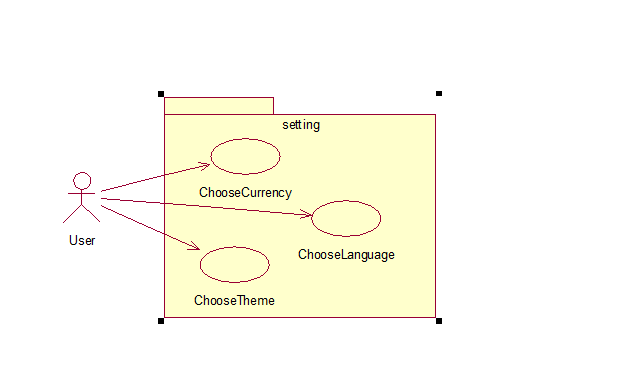
\includegraphics[scale=0.42]{setting部分用例图.png}
			\end{center}
			
			类图: 
			\begin{center}
			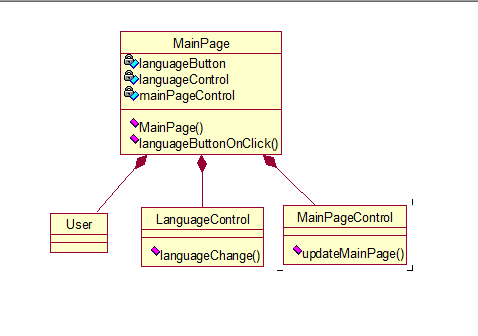
\includegraphics[scale=0.42]{选择语言类图.png}
			\end{center}

			状态图: 
			\begin{center}
			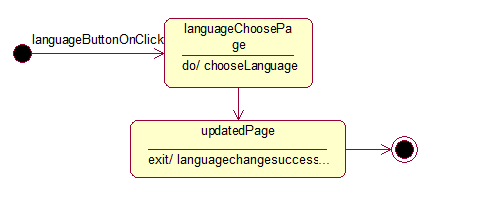
\includegraphics[scale=0.42]{选择语言状态图.png}
			\end{center}

			顺序图: 
			\begin{center}
			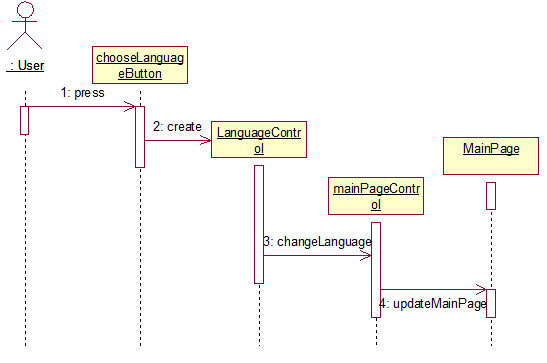
\includegraphics[scale=0.42]{选择语言顺序图.png}
			\end{center}



		\subsubsection{主题选择}
			用例: \\ \\
			\begin{tabular}{c|l}
			\hline
			用例名称 & 主题选择 Choose\ Theme \\ \hline
			参与者 & 用户 User  \\ \hline
			入口条件 & 用户 User 点击 主题选择按钮 \\ \hline
			事件流 & 	\parbox{33em}{\ \\
						1. 用户 User  点击主题选择按钮 \\
						2. Booking系统返回主题选择界面 \\
						3. 用户选择喜欢的主题并点击  \\
						4. 页面刷新, 并生成相应的主题界面 \\
						} \\ \hline
			出口条件 & \parbox{33em}{\ \\
						界面主题更换 \\
						} \\ \hline
			\end{tabular} \\ \\ \\
			\texttt{
			Algorithm Choosetheme:\\
			Input: selected theme(the theme which the user selected), the theme set, the set of URLs in different themes \\
			Output: null \\
			1: for each theme in the theme set do \\
			2:	if current theme == selected theme \\
			3:		address←URL in selected theme \\
			4: end for \\
			5: refresh the page \\
			6: return null \\
			} \\

			语言成分分析: \\
			\begin{center}
			\begin{tabular}{|c|c|c|}
			\hline
			语言成分 & 模型构件 & 实例\\ \hline
			专有名词 & Object & Jack  \\ \hline
			普通名词 & Class & 用户, 界面 \\ \hline
			Doing 动词 & Method &  点击, 更新, 刷新 \\ \hline
			名词 & Attribute & 主题图标按钮 \\ \hline
			\end{tabular}
			\end{center}

			用例图:
			\begin{center}
			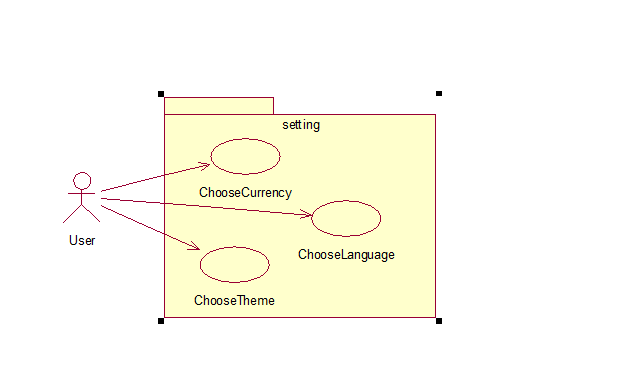
\includegraphics[scale=0.42]{setting部分用例图.png}
			\end{center}

			类图: 
			\begin{center}
			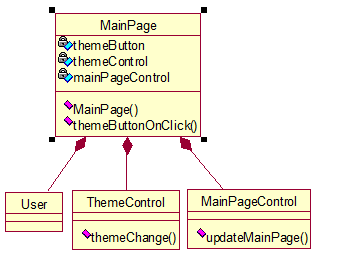
\includegraphics[scale=0.42]{选择主题类图.png}
			\end{center}

			状态图: 
			\begin{center}
			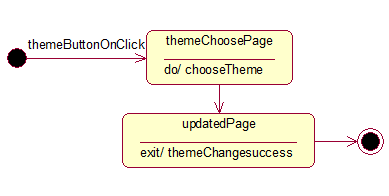
\includegraphics[scale=0.42]{选择主题状态图.png}
			\end{center}

			顺序图: 
			\begin{center}
			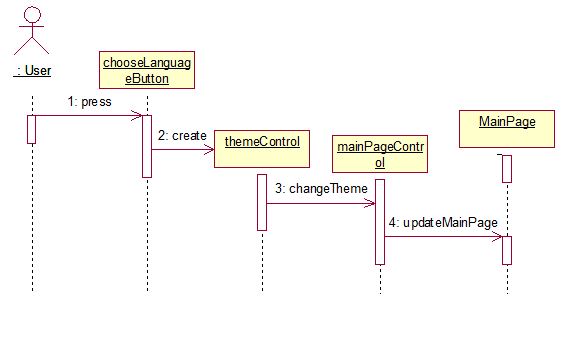
\includegraphics[scale=0.42]{选择主题顺序图.png}
			\end{center}


		\subsubsection{货币选择 Choose\ Currency}
			用例: \\ \\
			\begin{tabular}{c|l}
			\hline
			用例名称 & 货币选择 Choose\ Currency \\ \hline
			参与者 & 用户 User  \\ \hline
			入口条件 & 用户 User 点击货币选择按钮 \\ \hline
			事件流 & 	\parbox{33em}{\ \\
						1. 用户 User  点击货币选择按钮 \\
						2. Booking系统返回货币选择界面 \\
						3. 用户选择相应货币,点击确认  \\
						4. Booking系统保存相关设置到数据库中,刷新相应数据 \\
						5. 用户点击退出按钮 \\
						} \\ \hline
			出口条件 & \parbox{33em}{\ \\
						用户点击退出按钮 \\
						} \\ \hline
			质量需求 & \parbox{33em}{\ \\
						1. 网络通畅 \\
						2. 当前用户处于登录状态 \\
						} \\ \hline
			\end{tabular} \\ \\ \\
			\texttt{
			Algorithm Choose Currency \\
			Input : null \\
			Output : true or false \\
			1. if save successfully \\
			2.     return true \\
			3. else \\
			4.     return false \\
			} \\
			
			语言成分分析:
			\begin{center}
			\begin{tabular}{|c|c|c|}
			\hline
			语言成分 & 模型构件 & 实例\\ \hline
			专有名词 & Object & Jack  \\ \hline
			普通名词 & Class & 用户, 界面 \\ \hline
			Doing 动词 & Method &  显示, 修改, 检查, 保存 \\ \hline
			Having 动词 & aggregation & 包括 \\ \hline
			形容词, 名词 & Attribute & 货币类型 \\ \hline
			\end{tabular}
			\end{center}
			
			用例图:
			\begin{center}
			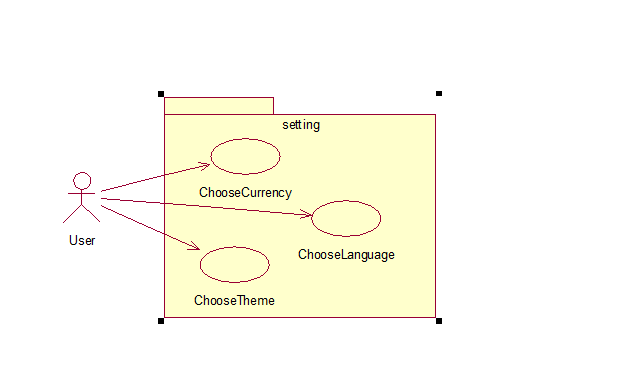
\includegraphics[scale=0.42]{setting部分用例图.png}
			\end{center}
			
			类图: 
			\begin{center}
			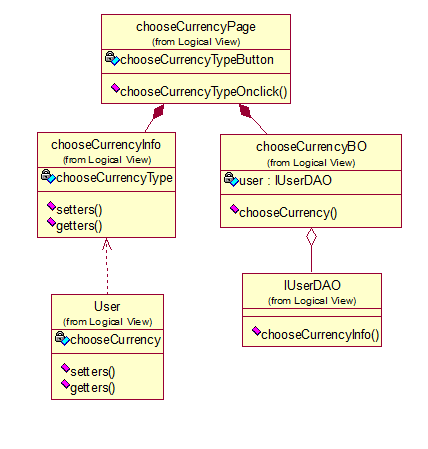
\includegraphics[scale=0.42]{选择货币类图.png}
			\end{center}

			状态图: 
			\begin{center}
			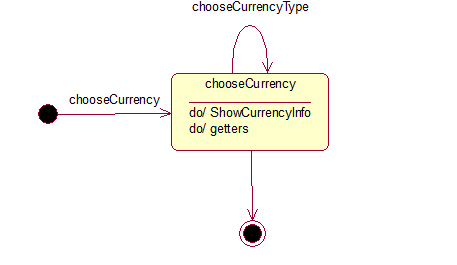
\includegraphics[scale=0.42]{选择货币状态图.png}
			\end{center}

			顺序图: 
			\begin{center}
			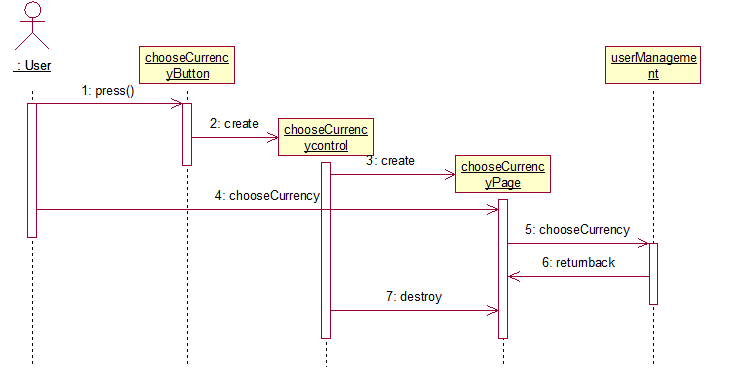
\includegraphics[scale=0.42]{选择货币顺序图.png}
			\end{center}


	\subsection{其他服务}
		\subsubsection{租车服务}
			用例: \\ \\
			\begin{tabular}{c|l}
			\hline
			用例名称 & 租车服务 Car\ Rental \\ \hline
			参与者 & 顾客 User  \\ \hline
			入口条件 & 用户点击租车按钮 \\ \hline
			事件流 & 	\parbox{33em}{\ \\
						1. 用户点击租车按钮 \\
						2. 系统弹出租车信息界面, 界面中含有起点, 终点, 预计时长, 预计消费, 以及附近车辆 \\
						3. 用户在页面中输入终点, 点击租车  \\
						4. 系统通知附近车辆, 等待司机选择接受 \\
						5. 如果用户在司机接受前点击取消, 则系统撤回通知, 租车结束 \\
						6. 司机选择接受, 系统撤回通知, 并通知用户司机已选择及司机的信息 \\
						7. 用户等待司机到达 \\
						8. 司机到达后, 用户搭乘司机车辆 \\
						9. 车辆到达指定地点, 司机点击结算 \\
						10. 租车结束 \\
						} \\ \hline
			出口条件 & 租车结束或者用户主动取消租车 \\ \hline
			\end{tabular} \\ \\ \\
			\texttt{
			Algorithm Car Rental \\
			Input : null \\
			Output : null \\
			1. jump to car rental page \\
			2. return null
			} \\
			
			语言成分分析:
			\begin{center}
			\begin{tabular}{|c|c|c|}
			\hline
			语言成分 & 模型构件 & 实例\\ \hline
			专有名词 & Object & Jack  \\ \hline
			普通名词 & Class & 用户、界面 \\ \hline
			Doing 动词 & Method &  点击、进入 \\ \hline
			名词 & Attribute & 按钮 \\ \hline
			\end{tabular}
			\end{center}
			
			用例图: 
			\begin{center}
			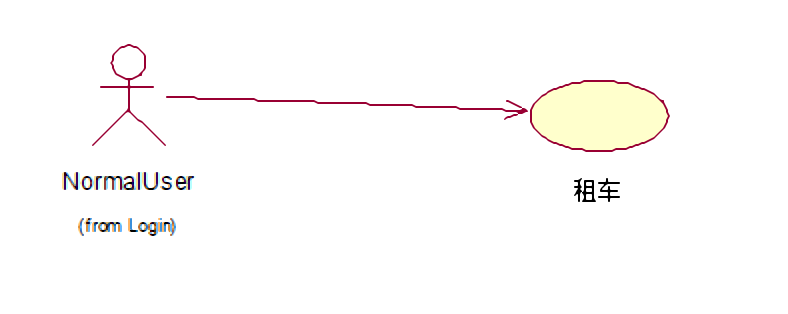
\includegraphics[scale=0.42]{租车服务_用例图.png}
			\end{center}

			类图: 
			\begin{center}
			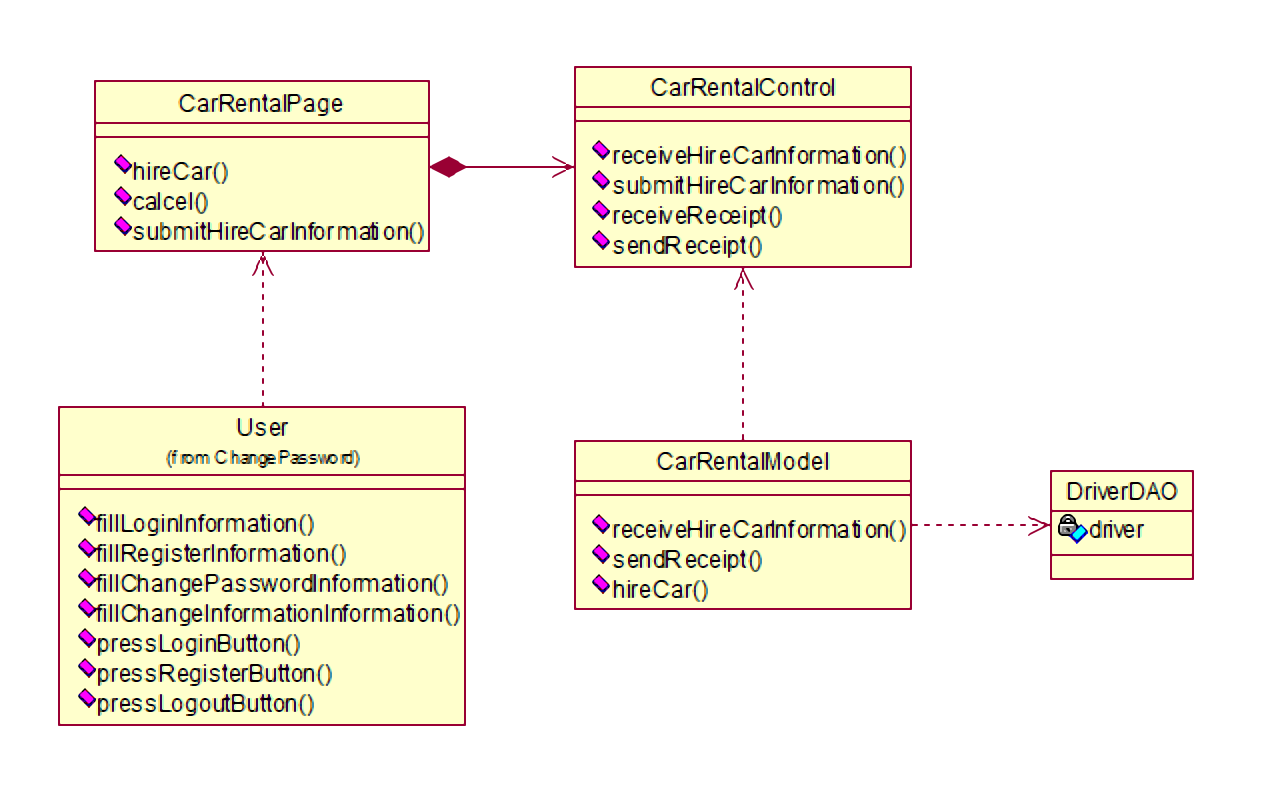
\includegraphics[scale=0.42]{租车服务_类图.png}
			\end{center}

			状态图: 
			\begin{center}
			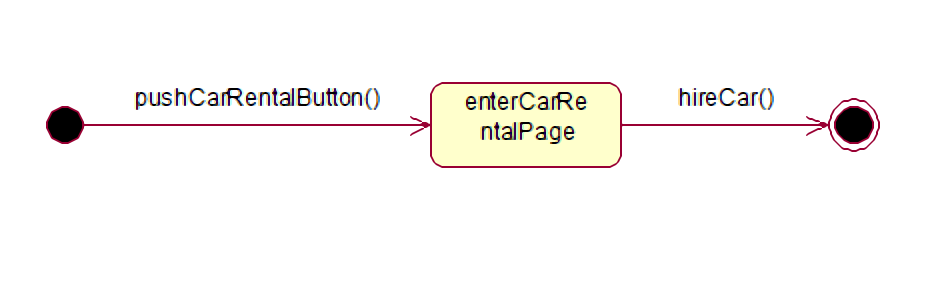
\includegraphics[scale=0.42]{租车服务_状态图.png}
			\end{center}

			顺序图: 
			\begin{center}
			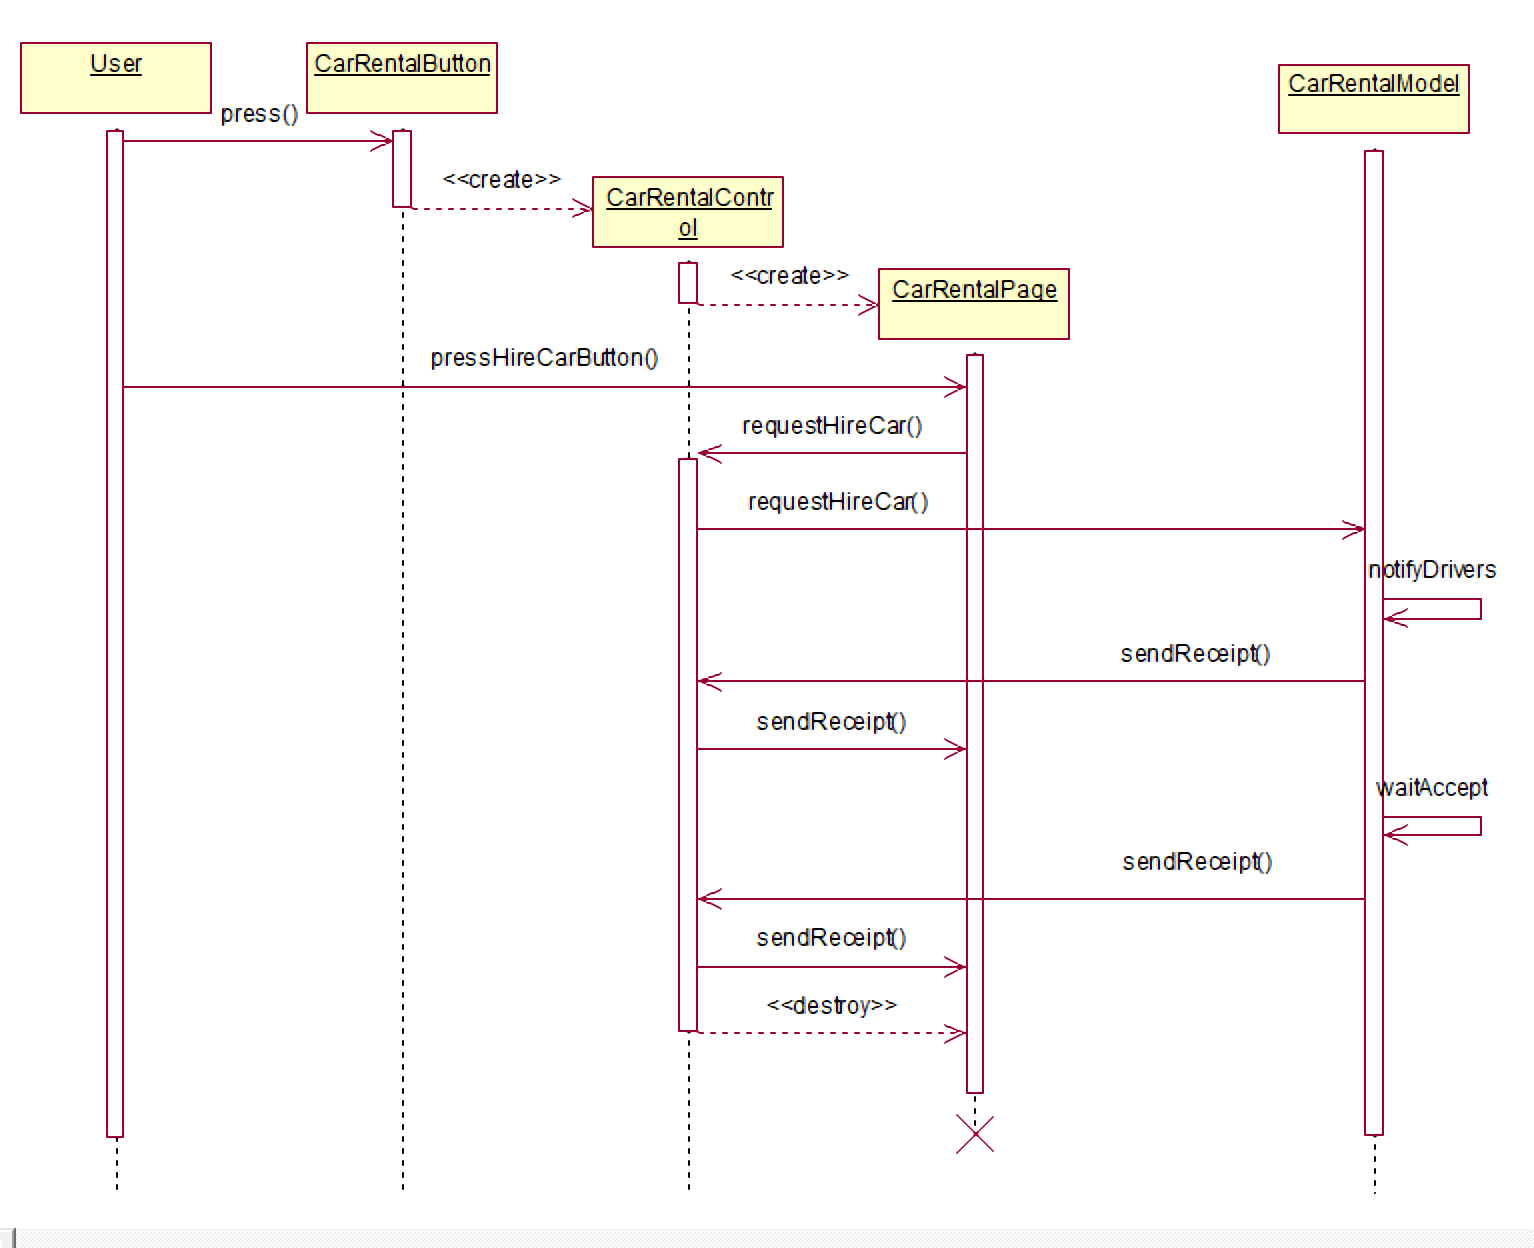
\includegraphics[scale=0.42]{租车服务_顺序图.png}
			\end{center}
			
			
		\subsubsection{餐厅订位 Reserve\ Restaurant}
			用例: \\ \\
			\begin{tabular}{c|l}
			\hline
			用例名称 & 餐厅订位 Reserve\ Restaurant \\ \hline
			参与者 & 顾客 User  \\ \hline
			入口条件 & 顾客点击餐厅订位按钮 \\ \hline
			事件流 & 	\parbox{33em}{\ \\
						1. 顾客点击餐厅订位按钮 \\
						2. 跳转到餐厅订位网站 \\
						} \\ \hline
			出口条件 & 进入餐厅订位网站 \\ \hline
			质量需求 & 网络通畅 \\ \hline
			\end{tabular} \\ \\ \\
			\texttt{
			Algorithm Reserve Restaurant \\
			Input : null \\
			Output : null \\
			1. jump to Reserve Restaurant page \\
			2. return null
			} \\
			
			语言成分分析:
			\begin{center}
			\begin{tabular}{|c|c|c|}
			\hline
			语言成分 & 模型构件 & 实例\\ \hline
			专有名词 & Object & Jack  \\ \hline
			普通名词 & Class & 用户、界面 \\ \hline
			Doing 动词 & Method &  点击、进入 \\ \hline
			名词 & Attribute & 按钮 \\ \hline
			\end{tabular}
			\end{center}
			
			用例图: 
			\begin{center}
			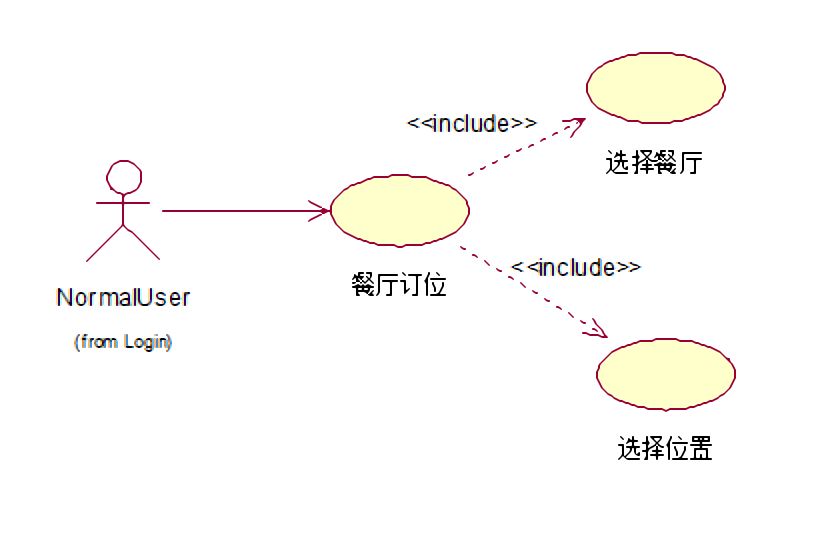
\includegraphics[scale=0.42]{餐厅订位_用例图.png}
			\end{center}

			类图: 
			\begin{center}
			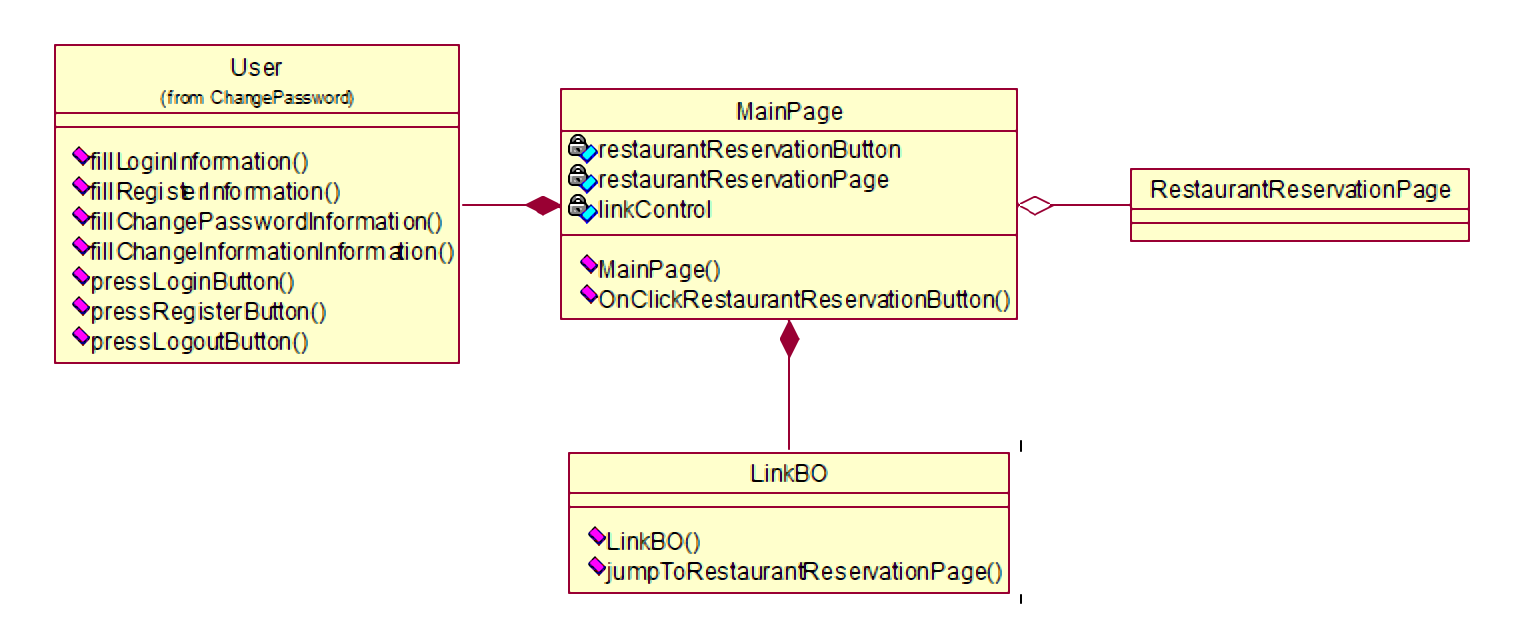
\includegraphics[scale=0.42]{餐厅订位_类图.png}
			\end{center}

			状态图: 
			\begin{center}
			\includegraphics[scale=0.42]{餐厅订位_状态图.png}
			\end{center}

			顺序图: 
			\begin{center}
			\includegraphics[scale=0.42]{餐厅订位_顺序图.png}
			\end{center}
			
\end{document}
